
%\parindent=0mm
%\parskip=10pt
\chapter{物件導論\\(Introduction to Objects)}\marginpar{\fbox{29}}
\begin{verse}
電腦革命始於機器。因此,程式語言的發軔也始於對機器的模仿。
\end{verse}

不過,電腦並非是那麼冷冰冰的機器。電腦是意念發揮的工具
(一如 Steve Jobs 常喜歡說的「意念的自行車」一樣),
並且也是一種不同類型的表達媒介。這個工具愈偏離機器的長相,
就愈像我們頭腦的一部份,一如寫作、繪畫、雕刻、動畫、電影等意念表達形式。
物件導向程式設計 (Object-oriented Programming,OOP),
便是這樣一個以電腦做為表達媒介的巨大浪潮中的一環。

本章將為你介紹基本的 OOP 觀念,並涵括軟體開發方法的概論性介紹。
本章,甚至整本書,都假設你對程序性語言
(procedural programming language)有著某種程度的經驗,我所謂程序性語言不一定得是
C。如果你覺得有必要在接觸此書之前先在程式設計和C 語法上多下功夫,
你可以研讀本書所附的培訓光碟《Thinking in C: Foundations for C++》,
其內容也可以從 www.BruceEckel.com 取得。
 
本章提供的是背景性、補充性的材料。
許多人在沒有看清整個物件導向程式設計方法的完整面貌之前,
無法自在地從事此類設計活動。因此,我將引入許多觀念,為你奠定 OOP 的紮實基礎。
另外還有許多人在沒有看到某種程度的實際運作機制之前,
無法看清物件導向程式設計方法的完整面貌。這樣的人如果沒有程式碼在手,
很容易迷失方向。如果你正是這種人,而且渴望早點知道Java 語言的細節,
請你從容跳過本章,這並不會影響你的程式撰寫和語言學習。不過,相信我,
最終你還是需要回過頭來填補必要的知識,藉以了解物件的重要,
以及「透過物件進行設計」的方式。

\section{抽象化的過程 (The progress of abstraction)}\marginpar{\fbox{30}}
所有程式語言都提供抽象化機制 (abstraction)。甚至可以大膽地說,
我們所能解決的問題的複雜度,取決於抽象化的類型和品質。我所謂類型,
指的是「你所抽象化的事物為何?」組合語言僅對底層的實體機器進行少量抽象化。
許多所謂命令式(imperative)程式語言(例如Fortran、
BASIC、C),則在組合語言之上再抽象化。此類語言大幅改進了組合語言,
但它們所做的主要是機器本身的抽象化,
你依舊無法逃脫「以電腦結構進行問題思考」的命運,
因而無法以待解問題的結構來做為思考基準。
程式設計者必須自行建立介於機器模型(位於你所建立之問題模型的解域
(solution space,例如電腦)內)和實際待解問題模型(位於問題實際存在之題域
(problem space) 內) 之間的關聯性。這裡頭需要的便是「對映
(mapping)」功夫,然而這種能力並非程式語言的自性本質,這使得程式難以撰寫,
維護代價高昂。於是才產生出「程式方法(programming methods)」這個產業。

另一種建立機器模型的方式,便是建立待解問題的模型。早期的程式語言如
LISP 和APL 都選擇了觀看世界的某種特定方式,
分別認為「所有的問題最終都是lists」、「所有的問題都是演算形式(algorithmic)」。
PROLOG 則將所有問題轉換為一連串決策(chains of decisions)。另外也有基於制約條件
(constraint-based) 的程式語言,以及專門處理圖形化符號的程式語言
(後者已被證明束縛太多)。這些方式對於它們所瞄準的特定題型,
都能提供不錯的解決方案,然而一旦跳脫特定領域,就顯得時地不宜。

物件導向法(Object Oriented approach)更進一步,提供各式各樣的工具,
讓程式設計者得以在題域 (problem space) 中表現必要的元素。
這種\marginpar{\fbox{31}}表達方式具備足夠的一般化,
使程式設計者不必受限於任何特定題型。我們將題域中的元素和其在解域
(solution space) 中的表述 (representation)稱為「物件」
(當然你還需要其他一些無法被類比為題域內的元素的物件)。
這其中的觀念是,程式可以透過「導入新型物件」
而讓自己得以適用於特定領域的問題;當你閱讀解法的程式碼時,
便如同閱讀問題本身的表述一樣。
這種語言比我們過去所擁有的任何語言具備更彈性更威力的抽象化機制。
因此OOP 提供了以問題描述問題(describe the problem in terms of the problem)
的能力,而不再是以解答執行之所在(電腦)的形式來描述問題。不過,當然了,
最終還是會接回電腦本身。每個物件看起來都有點像是一部微型電腦,有著自身的狀態,
你也可以要求執行它所提供的種種操作(operations)。如果把它們類比至真實世界,
以這種角度來說似乎不錯:它們都有特性(characteristics)和行為 (behaviors)。

有些程式語言設計者認為,單靠物件導向程式設計本身,
還不足以輕易解決所有程式設計問題,
因而倡議所謂的「多模式(multiparadigm)」程式語言,
試圖融合多種不同的解決方案\footnote{請參考Timothy Budd,《Multiparadigm
Programming in Leda》,Addison-Wesle,1995.}。

Alan Kay 曾經摘要整理了Smalltalk 的五大基本特質。而Smalltalk 正是第
一個成功的物件導向程式語言,同時也是Java 以為根基的語言之一。
Smalltalk 的特性代表物件導向程式設計最為純淨的一面:
\begin{enumerate}
\item 萬事萬物皆物件。將物件視為神奇的變量,除了可以儲存資料之外,
你還可以「要求」它執行自身所具備的操作能力。
理論上你可以將待解問題中的所有觀念性組成,都變成程式中的物件。
\item 程式便是成堆的物件,彼此透過訊息的傳遞,請求其他物件進行工作。
如果想對物件發出請求(request),你必須「傳送訊息」至該物件。
更具體地說你可以把訊息想像是對「隸屬某個特定物件」的函式的呼喚請求。
\item
每個物件都擁有由其他物件所構成的記憶。
你可以藉由「封裝既有\marginpar{\fbox{32}}物件(s)」的方式來產生新型態的物件。
因此你可以在程式中建立複雜的體系,卻將複雜的本質隱藏於物件的單純性之下。
\item 每個物件皆有其型別( type ) 。就像「每個物件皆為其類別
(class)的一個實體(instance)」這種說法一樣,類別(class)
即型別(type)的同義詞。不同的類別之間最重要的區分就是:
你究竟能夠發送什麼訊息給它?
\item 同一型別的所有物件接受的訊息皆相同。這句話在稍後還會陸續出現。
由於「圓形」物件同樣也是「幾何形」物件,
所以「圓形」肯定能接受所有可以發送給「幾何形」的訊息。
這意謂你可以撰寫和「幾何形」溝通的程式碼,
並自動處理所有與「幾何形」性質相關的事物。
這種「替代能力(substitutability)」正是OOP 中最具威力的概念之一。
\end{enumerate}
\section{每個物件都有介面 \\(An object has an interface)}
亞理斯多德或許是第一個深入考究「型別(type)」的哲人;他曾提過魚類和鳥類
(the class of fishes and the class of birds)
這樣的字眼。史上第一個物件導向程式語言 Simula-67,則是透過基礎關鍵字 class,
將新型別導入程式中,從而直接引用了類別的概念。這個概念是:
所有物件都是獨一無二的,但也都是「屬於同一類別、
有著共同特性和行為」之所有物件的一部份。

Simula,一如其名,誕生目的是為了發展模擬程式。
例如古典的「銀行出納員問題」中存在許多出納員、客戶、帳號、交易、以及金錢單位,
這正是許多「物件」的寫照。
「隸屬同一類別」的眾多物件除了在程式執行期具備不同的狀態外,其餘完全相同,
這也正是class 這個關鍵字的由來。 建立抽象資料型別(類別),
是物件導向程式設計中的基本觀念。
抽象資料型別的運作方式和內建基本型別幾乎沒什麼兩樣。
你可以產生隸屬某個\marginpar{\fbox{33}}型別的變數
(以物件導向的說法,此可稱為物件或實體,instance),也可以操作這些變數
(這種行為亦稱為「遞送訊息」或「發出請求」;是的,
你送出訊息,物件便能夠知道此訊息相應的目的)。每個類別的成員
(members),或稱為元素(elements),都共用相同的性質,例如每個帳戶都有結餘金額,
每個出納員都能夠處理存款動作...等等。此外,每個成員也都有其自身狀態,
例如每個帳戶都有不同的結餘金額,每個出納員都有各自的姓名。於是出納員、客戶、
帳戶、交易等等在電腦中都可以被表現為獨一無二的個體。這樣的個體便是物件,
每個物件都隸屬於特定的類別,該類別定義了物件的特性和行為。

所以,雖然我們在物件導向程式設計過程中,實際所做的是建立新的資料型別
(data types),但幾乎所有物件導向程式語言都使用 class 這個關鍵字來表示 type。
當你看到型別(type)一詞時,請想成是類別 (class),
反之亦然\footnote{某些人對此還是有所區別,他們認為 type 決定了介面
(interface),而class 則是該介面的一個特定實作品。}。
由於 class 描述了「具有共同特性(資料元素)和共同行為(功能)」的一組物件,
所以 class 的的確確就是data type,就像所有浮點數都有一組共通的特性和行為一樣。
箇中差異在於,程式設計者藉由定義class 以適應問題,
而不再被迫使用那些現成的data types -
它們僅僅被設計用來表示機器中的某個儲存單元。你可以針對自己的需求,加入新的
data types,因而擴展程式語言的功能。程式設計系統欣然接受新的 classes,
同時也賜予它們和內建 types 一樣的照料及一樣的型別檢驗 (type- checking)。

物件導向方法並不侷限於模擬程式的發展。
無論你是否同意「所有程式都是用來模擬你正在設計的那個系統」這一論點,OOP
技術都可以輕易簡化許多大型問題,得到簡單的解決方案。

一旦 class 建立之後,隸屬該 class 的物件,你想要多少個就能產生多少個。
你可以操作這些物件,就像它們是存在於待解問題中的元素一般。

確實,\marginpar{\fbox{34}} 物件導向程式設計的挑戰之一,
便是在題域內的眾多元素與解域內的眾多物件之間,建立起一對一的對映。

現在,問題來了,你該如何令物件為你所用呢?必須有某種方式對物件發出請求,
使物件能夠做些諸如完成一筆交易、在螢幕上繪圖、打開某個開關之類的工作。
每個物件都只能滿足某些請求。物件的介面(interface)
定義了它所接受的請求內容,而決定介面的便是type(型別)。
我們可以拿電燈泡做一個簡單的比喻:

\begin{figure}[htbp]
\centering
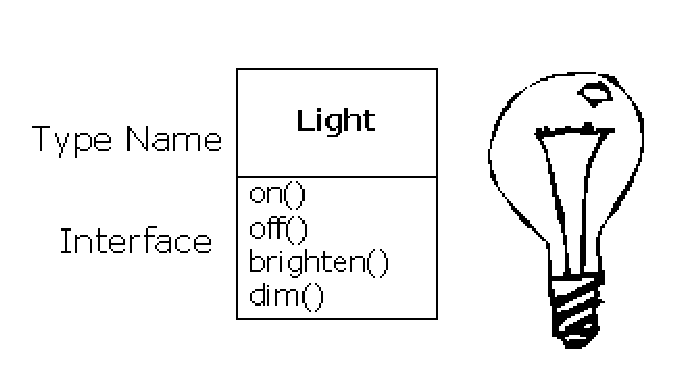
\includegraphics[scale=0.8]{eps/TIJ203.eps}
\end{figure}

\begin{verbatim}
Light lt = new Light();
lt.on();
\end{verbatim}

介面(interface)規範了你能夠對物件發出的請求。不過,
還是得有程式碼來滿足這些請求。這些程式碼加上被隱藏的資料,構成所謂的實作
(implementation)。從程序式設計(procedural programming)的觀點來看,
並沒有太複雜。每個type 都有一些函式對映於任何可能收到的請求。
當你對某個物件發出某個請求,某個函式便被喚起。此一過程通常被扼要地說成:
你送出訊息(發出請求)至某物件,該物件便知道此一訊息的對應目的,
進而執行起對應的程式碼。

本例之中的 type/class 名稱是 Light,特定的 Light 物件名為 lt。你能夠對
Light 物件發出的請求是:將它打開、將它關閉、使它亮些、使它暗些。
本例產生一個Light 物件的方式是:定義lt 這個物件名稱,並呼叫
new 請求產生該種型別的物件。欲發送訊息給物件,可以先標示出物件名稱,
再以句點符號(dot)連接訊息請求。從使用者的觀點出發,
這種「以物件來進行設計」的型式很漂亮。

上圖\marginpar{\fbox{35}}是以所謂 UML(Unified Modeling Language)形式呈現:
每個 class 皆以矩形方格表示,class/type 名稱位於方格上方,你所關心的任何 data
members(資料成員)都置於方格中央,方格下方放置所謂的 member functions
(成員函式),這些函式隸屬於此一物件,能夠接收你所發送的
訊息。通常只有class 名稱及公開的(public)member functions 會被顯示
於UML 圖中,方格中央部份不繪出。如果你只在意class 名稱,那麼甚至
方格下方的部份也沒有必要繪出。
\section{被隱藏的實作細節 \\(The hidden implementation)}
將程式開發人員依各自的專業領域加以區分,對我們的概念釐清大有幫
助。程式開發人員可分為:開發新資料型別的所謂class 創造者,以及在應
用程式中使用他人所開發之classes 的所謂客端程式員
( client programmers)\footnote{關於這個詞彙的使用,我得感謝我的朋友 Scott
Meyers。}。 客端程式員的目標是收集許多可供運用的classes 以利快速開發應用程式。
Class 創造者的目標則是打造classes,並且只曝露客端程式員應該知道的事物,
隱藏其他所有事物。為什麼?因為如果加以隱藏,客端程式員便無法使用,
這意謂class 創造者可以改變隱藏的部份,不必擔心對其他人造成衝擊。
隱藏部份通常代表物件內部脆弱的一環,
它們很容易被不小心或不知情的客端程式員毀壞掉。
因此將實作部份隱藏起來可以減少程式臭蟲。實作隱藏(implementation hiding)
的觀念再怎麼強調也不過份。

在任何相互關係中,存在一個「參與者共同遵守的界限」是一件重要的事情。
當你建立一個class library 時,你會和客端程式員建立起關係。
他可能在某個程式中使用你的library,也可能建立一個更大的library。
如果\marginpar{\fbox{36}}任何人都可以取用某個 class 的所有members,
那麼客端程式員便可以對 class 做任何事情,不受任何管束。
你可能希望客端程式員不要直接操作你的class 中的某些 members,
但如果缺少某種「存取權限控管機制」,就無法杜絕此事,
導致每個物件都赤裸裸地攤在陽光下。

因此,「存取權限控管機制」的第一個存在理由便是,
讓客端程式員無法碰觸他們不該碰觸的事物 - 這些部份應該僅供
data type 內部使用,而非被外界用來解決特定問題。
這對使用者而言其實也是一種服務,因為使用者可以輕易看出哪些事物對他們來說重要,
哪些可以忽略。

「存取權限控管機制」的第二個存在理由是,讓library 設計者得以改變
class 內部運作方式而不擔心影響客端程式。舉例來說,你可能想要簡化開發動作,
改以較簡單的方式來實作某一特定class。但稍後卻發現,
你得重新寫過才能改善其執行速度。如果介面和實作二者能夠切割清楚,
這個工作便輕而易舉。

Java 使用三個關鍵字來設定class 的存取界限:public、private、
protected。這些關鍵字的意義和用法相當直覺。這些被稱為「存取指定詞
(access specifiers)」的關鍵字,決定了誰才有資格使用其下所定義的東西。
接續在 public 之後的所有定義,每個人都可取用。接續在 private 之後的所有定義,
除了型別開發者可以在該型別的 member functions 中加以取用,
沒有其他任何人可以存取。private 就像是你和客端程式員之間的一堵牆,
如果有人企圖存取private members,會得到編譯期錯誤訊息。protected 和
private 很相像,只不過class 繼承者有能力存取 protected members,卻無法存取
private member。稍後還會有對繼承 (inheritance)的簡短介紹。

Java 還有一種所謂的「預設(default)」存取權限。
當你沒有使用上述任何一個指定詞時,用的便是這種存取權限。有時候這被稱為
friendly 存取權限,因為同一個 package 中的其他classes,
有能力存取這種所謂的 friendly members,但在 package 之外,這些 friendly members
形同 private members。

\section{重複運用實作碼 \\(Reusing the implementation)}\marginpar{\fbox{37}}
一旦 class 開發完成並經測試,它應該(理想情形下)代表著一份有用的程式單元
(unit of code)。雖然很多人都對復用性(reusability)有著熱切的期望,但事實證明,
欲達此目的並不容易,你得具備豐富的經驗和深刻的見解。一旦某個 class
具備了這樣的設計,它便可以被重複運用。程式碼的重複運用,
是物件導向程式設計所提供的最了不起的優點之一。

想要重複運用某個class,最簡單的方式莫過於直接使用其所產生的物件。
此外你也可以把某個class 物件置於另一個class 內。我們稱這種形式為
「產生一個成員物件」。新的classes 可由任意數目、任意型別的它種物件組成,
這些物件可以任何組合方式達到你想要的功能。由於這種方式是「以既有的
classes 合成新的class」,所以這種觀念被稱為「複合
(composition)」或「聚合(aggregation)」。複合通常被視為 ``has-a''
(擁有)的關係,就好像我們說「車子擁有引擎」。

\begin{figure}[htbp]
\centering
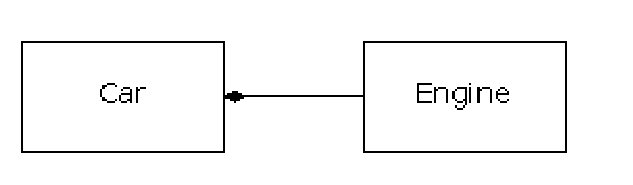
\includegraphics{eps/TIJ204.eps}
\end{figure}

(以上UML 圖以實心菱形指向車子,代表複合關係。我通常採用更簡單的形式,
只畫一條線而不繪出菱形, 來代表聯繫 (association)
關係\footnote{在大多數示意圖中,這樣的表示便已足夠,
通常你不需要在意使用的究竟是聚合或是複合。}。

透過複合,程式員可以取得極大彈性。class 的成員物件通常宣告為
private,使客端程式員無法直接取用它們。
這也使你得以在不干擾現有\marginpar{\fbox{38}}客戶程式碼的情形下,
更動這些成員。你也可以在執行期改變成員物件,
藉以動態改變程式行為。稍後即將探討的「繼承(inheritance)」關係,
由於編譯器會對透過繼承而產生的class 加上諸多編譯期限制,
因此繼承不具備這樣的彈性。

由於繼承在物件導向程式設計中如此重要,使得它常常被高度地、
甚至過度地強調。程式設計新手於是會有一種刻板印象,
以為「應該處處使用繼承」。這會造成誤用,並導致過於複雜的設計。
事實上在建立新class 時, 你應該先考慮複合(composition),
因為它夠簡單又具彈性。如此一來你的設計會更加清晰。有了一些經驗之後,
便更能看透繼承的必要運用時機。
\section{繼承:重複運用介面 \\ Inheritance: reusing the interface}
物件這個觀念, 本身就是十分好用的工具, 讓你得以透過概念
(concepts) 將資料和功能封裝在一起, 因而表述出題域( problem
space)中的想法,不必受迫於使用底層機器語言。這些概念係以關鍵字
class 來表現,成為程式語言中的基本單位。

可惜的是,這樣還是有許多麻煩:建立某個class 之後,即使另一個新的
class 有著相似功能,你還是被迫重頭建立新的class。如果我們能夠站在既有基礎上,
複製class 的內容,然後這邊加加、那邊改改,可就真是太好了。
事實上透過繼承便可達到如此的效果。不過有個例外:當原先的class
(稱為base class 或super class 或parent class)發生變動時,修改過的
「複製品」(稱為derived class 或inherited class 或sub class 或child
class)也會同時反映這些變動。

\marginpar{\fbox{39}}
\begin{figure}[htbp]
\centering
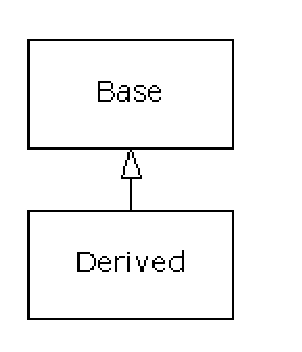
\includegraphics{eps/TIJ205.eps}
\end{figure}

(以上UML 圖中的箭號,是從derived class 指向base class。稍後你便能夠理解,
可以存在一個以上的derived classes。)

type 不僅僅只是用來描述一組物件的制約條件,同時也具備了與其他types
之間的關係。兩個types 可以有共通的特性和行為,但其中某個 type
也許包含較多特性,另一個 type 也許可以處理較多訊息
(或是以不同的方式來處理訊息)。所謂「繼承」便是透過 base types 和
derived types 的觀念,
表達這種介於type 和type 之間的相似性。Base type 內含所有derived
types 共享的特性和行為。你可以使用base type 代表系統中某些物件的核心概念,
再以base type 為基礎,衍生出其他types,
用來表示此一核心部份可被實現的種種不同方式。

以垃圾回收機(trash-recycling machine)為例,它用來整理散落的垃圾。
假設base type 是「垃圾」,那麼每一袋垃圾都有重量、價值等特性,
可被切成絲狀、可被熔化或分解。以此為基礎,
可以衍生出更特殊的垃圾型式,具備額外的特性(例如罐子可以有顏色)或行為
(鋁罐可壓碎、鐵罐具有磁性)。此外,它們的某些行為可能不同
(例如紙張的價值便和其種類與狀態有關)。透過繼承的使用,
你可以建立一個型別階層體系(type hierarchy),表現出你想要解決的問題。

第二個例子是經典的 shape (幾何形狀)範例,
可能用於電腦輔助設計系統或模擬遊戲之中。
Base type 便是 ``shape'',擁有大小、顏色、位置等特性,並且可被繪製、擦拭、
移動、著色。以此為基礎,便可衍生出各種特定的幾何形狀出來:圓形、正方形、
三角形...,每種形狀都可以擁有額外的特性和行為,例如某些形狀可以被翻轉。
某些行為也許並不相同,例如\marginpar{\fbox{40}}面積計算的方式便不盡相同。
型別階層體系(type hierarchy)同時展現了各種形狀之間的相似性和相異性。

\begin{figure}[htbp]
\centering
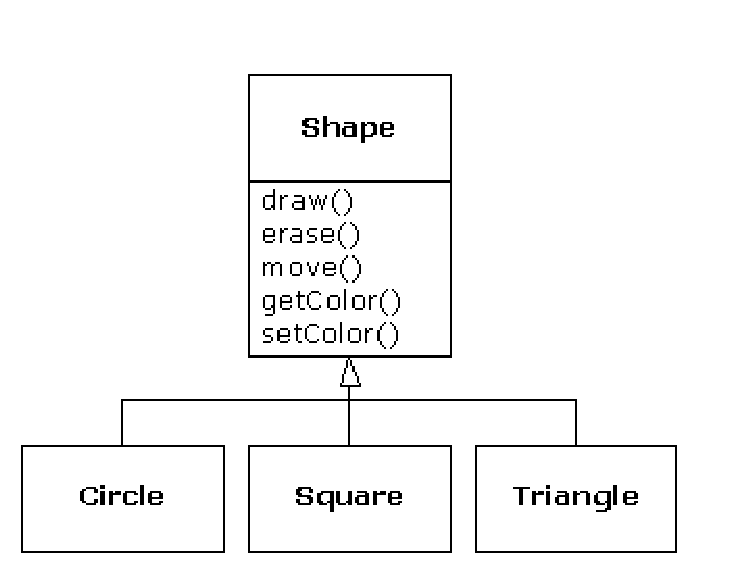
\includegraphics{eps/TIJ206.eps}
\end{figure}

如果我們能以問題原本所用的術語來轉換解答,將會大有益處,
因為你不需要在問題的描述和解答的描述之間,建立起眾多中介模型。
透過物件的使用,type hierarchy(型別階層體系)成了主要模型,
讓你得以直接自真實世界出發,以程式碼來描述整個系統。是的,
對使用物件導向程式設計的人們來說,眾多難以跨越的難關之一便是,
從開始到結束太過於簡單。 對於一顆久經訓練、善於找尋複雜解答的頭腦來說,
往往會在接觸的一開始被這種單純特性給難倒。

當你繼承既有的type 時,便創造了新的type,後者不僅包含前者的所有成員
(但priavte 成員會被隱藏起來,而且無法存取),更重要的是它同時也複製了
base class 的介面。也就是說,所有可以發送給base class 物件的訊息,
也都同樣可以發送給derived class 物件。
由於我們可以透過「可發送之訊息型態」來得知物件的
type,因此前述事實告訴我們,derived class 和
base class 具有相同的type。
例如前一個例子中我們便可以說「圓形是一種幾何形狀」。
透過繼承而發生的型別等價性 (type equivalence),
是了解物件導向程式設計真髓的重要關鍵。

base class\marginpar{\fbox{41}} 和 derived class 有著相同的介面,
而一定有某些實作碼伴隨著此一介面。也就是說,當物件接收到特定訊息時,
還是得有程式碼來執行動作。倘若你只是很簡單地繼承了 class,
然後再沒有做任何事情,那麼 base class 的介面所伴隨的函式,
便會原封不動地被繼承到 derived class 去。這表示 derived class 物件不僅擁有與
base class 物件相同的型別(type), 也擁有相同的行為,這沒什麼趣味。

兩種作法可以產生 derived class 與 base class 之間的差異。第一種作法十分直覺,
只要直接在 derived class 中增加新函式即可。這些新函式並非 base class
介面的一部份。這意謂base class 無法滿足你的需要,因此你得加入更多函式。
這種既簡單又基本的方式,有時候對你的問題而言是一種完美解答。
但是你應該仔細思考,你的 base class 是否也可能需要這些額外功能。
這種發現與更替的過程,會在整個物件導向設計過程中持續發生。

\begin{figure}[htbp]
\centering
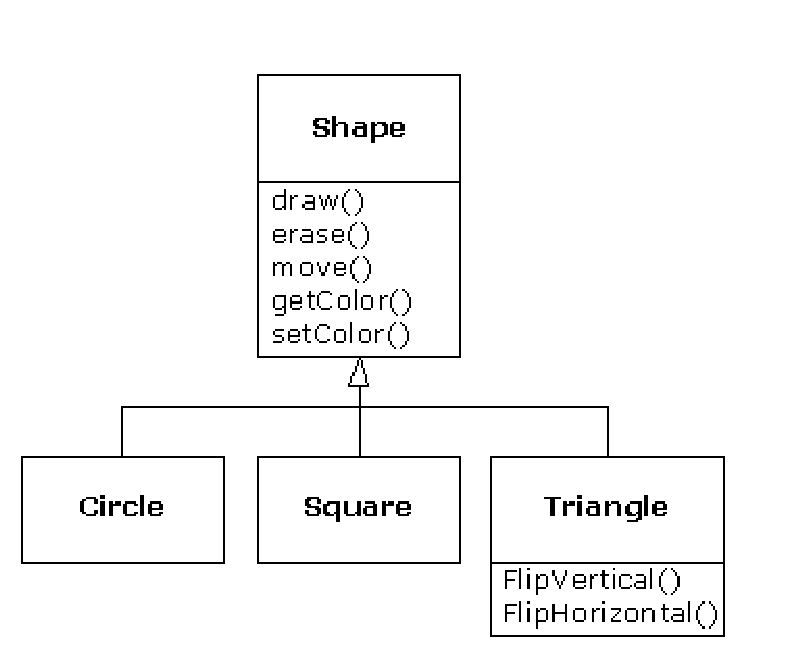
\includegraphics{eps/TIJ207.eps}
\end{figure}

雖然繼承有時候意味著加入新功能至介面中 (尤其 Java 更是以關鍵字
extends 代表繼承),但並非總是如此。
形成差異的第二種方法 (也許\marginpar{\fbox{42}}是更重要的方法)
便是改變既有之base class 的函式行為,這種行為我們通常稱為「覆寫(overriding)」。

\begin{figure}[htbp]
\centering
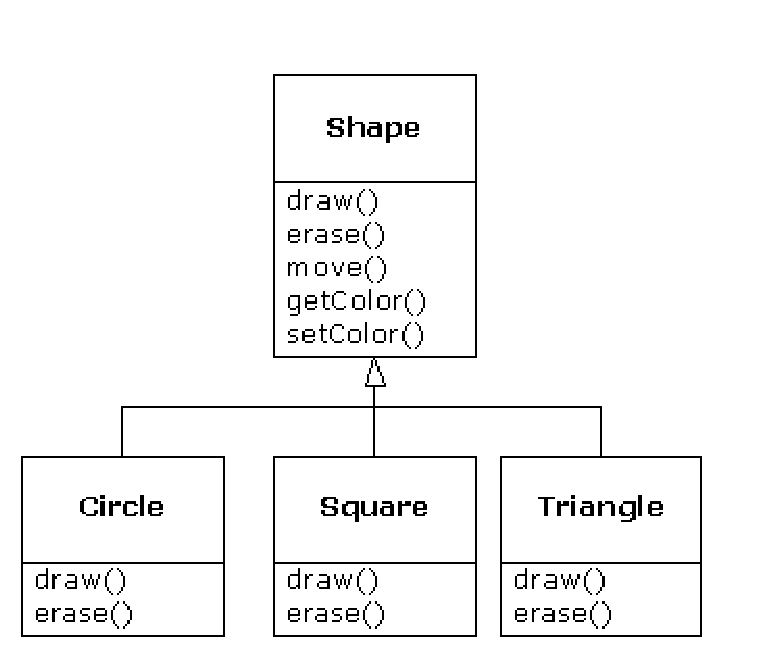
\includegraphics[scale=0.8]{eps/TIJ208.eps}
\end{figure}

想要覆寫某個函式,只須在 derived class 中建立該函式的一份新定義即可。
這個時候你的意思是:「在這裡我使用相同的介面函式,
但我想在新型別中做點不一樣的事情。」

\subsection{是一個(is-a)vs. 像是一個(is-like-a)}
繼承過程中可以進行的動作,仍舊有些爭論。繼承應該「只」覆寫 base
class 的函式(而不加入任何新函式)嗎?如果這樣,便意謂 derived class
和base class 有著完全相同的type,因為它們的介面一模一樣。這樣得到的結果是,
你可以以derived class 物件完全替換base class 物件。這可視為一種「純粹替代
( pure substitution ) 」, 通常稱為「替代法則
(substitution principle)」。就某種意義而言,這是處理繼承的一種理想方式。
我們通常將這種介於base class 和derived class 之間的關係稱為
「is-a(是一種)」關係,因為你可以說「圓形是一種幾何形狀」。
套用繼承關係與否的一個檢驗標準便是,你是否可以有意義地宣稱
classes 之間具備「is-a」的關係。

不過\marginpar{\fbox{43}}有些時候,你還是得將新的介面元素加到derived type 中,
如此也就擴充了介面,進而產生新的 type。新的 type 仍然可以替換 base type,
但這種形式的替換並非完美無瑕,因為 base type 無法取用你加入的新函式。
這種關係我們可以用「is-like-a(像一個)\footnote{這是我發明的詞彙。}」的方式描述。新type 具備和舊
type 相同的介面,但還包含其他函式,所以不能宣稱它們二者完全相同。
以冷氣機為例,假設你的房子裝設了給所有冷卻系統用的控制機制,
也就是說它具備讓你控制冷卻系統的介面。現在,冷氣機壞了,你新裝上一部冷暖氣機。
這個冷暖氣機便「is-like-a(像是一個)」冷氣機,但它可做的事情更多。
但因為房子的控制系統只能控制冷卻功能,所以只能夠和新物件中的冷卻部份溝通。
新物件的介面雖然擴充了,但舊系統除了原介面之外,完全不知道任何其他事情。

\begin{figure}[htbp]
\centering
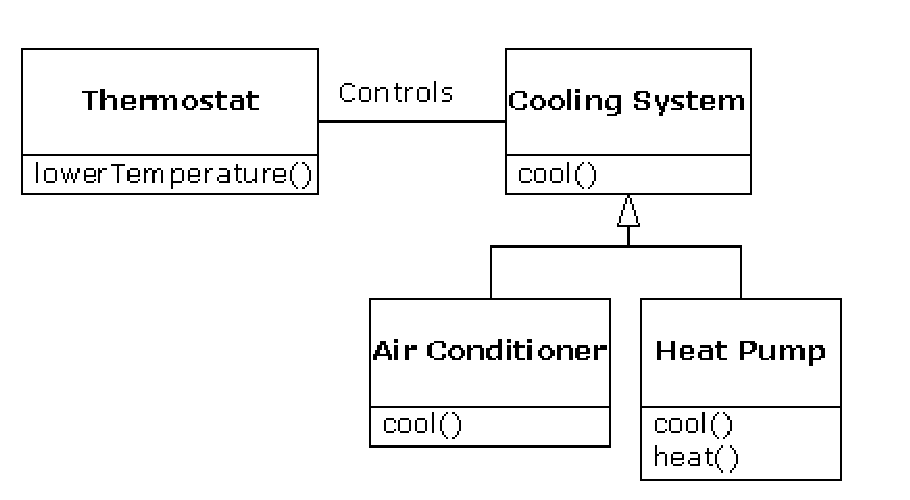
\includegraphics[scale=0.8]{eps/TIJ209.eps}
\end{figure}


當然,看過這樣的設計之後,你便會發現,base class 的「冷卻系統」不夠一般化,
應該改為「溫度控制系統」,使它得以涵蓋加熱功能 - 於是我們便可套用所謂
「替代法則」了。上圖是個範例,說明在設計領域和真實世界中可能發生的事情。

當你了解替代法則\marginpar{\fbox{44}} (substitution principle),
很容易便會以為「純粹替代」是唯一可行之道。事實上如果你的設計能夠依循此種方式,
是滿好的。不過偶而你還是會遭遇到「需要將新函式加入derived class 介面」
的情況。只要仔細檢閱,這兩種情形的使用時機應該是相當明顯的。

\section[隨多型而生的可互換物件]{隨多型而生的可互換物件 \\(Interchangeable objects with polymorphism)}
處理type 階層體系內的物件時,我們往往希望能夠不以它們所屬的特定
type 看待之,而以其base type 視之。如此一來我們所撰寫的程式碼便不會和特定的
type 有依存關係。以幾何形狀為例,用來操作一般化(泛化、
generic)形狀的函式,其實不需要在意其所處理的形狀究竟是圓形、正方形、三角形、
或其他尚未被定義的種種形狀。因為所有形狀都可以被繪製、被擦拭、被移動,
因此這些函式只需發送訊息給「形狀」物件,不需擔心對方怎麼處理這些訊息。

為了擴充物件導向程式的能力,以便處理新狀況,最常用的手法就是加入新
types。此類程式碼的特性就是,不會因為額外加入新型別而受到影響。
例如你可以衍生出幾何形狀的 subtype - 五邊形 (pentagon),
卻不需要修改任何函式 - 只要這些函式僅只處理泛化的(generic)幾何形狀。
這種「透過衍生新的subtype 而擴充程式能力」的手法相當重要,
因為這種能力可以大幅改善設計,使軟體的維護成本降低。

不過,完美的事物並不存在於人間。當我們試著以泛化的base type 來看待
derived type 物件時(例如以幾何形狀來看待圓形、以交通工具來對待腳踏車、
把鸕鶿看做是鳥等等),倘若某個函式要求某一泛化形狀繪製自己,
或是要求某個泛化交通工具前進,或是要求某隻泛化的鳥移動,
編譯器在編譯期便無法精確知道究竟應該執行哪一段程式碼。這是關鍵所在:
訊息被發送時,程式設計者並不想知道哪一段程式碼會被執行;繪圖函式施行於圓形、
正方形、三角形身上完全沒有兩樣,
物件執行時會依據自身的實際型別來決定究竟該執行哪一段程式碼。
如果「知道哪一段程式碼將被執行」對你而言並非必要,那麼當你加入新的子型別
(subtype)時,不需更動函式叫用句,就可以視子型別的不同而執行不同的程式碼。
也因此,編\marginpar{\fbox{45}}譯器無法精確知道究竟哪一程式碼會被執行起來。
那麼編譯器又做些什麼事呢?以下圖為例,BirdController 物件僅處理泛化的
Bird 物件,因此它「對那些Bird 物件實際上是什麼型別」毫不知情。從
BirdController 的角度來看,這麼做是十分方便的,
它將因此而不必撰寫特別的程式碼來判斷所處理的
Bird 物件究竟是什麼型別,也不需要判斷這些Bird 物件會有什麼特別行為。然而,
在忽略Bird 實際型別的情況下,當move() 被呼叫時,物件的實際行為會是什麼?鵝
(Goose)會用跑的還是飛的?還是游泳?企鵝(Penguin)會用跑的還是游水的方式?

\begin{figure}[htbp]
\centering
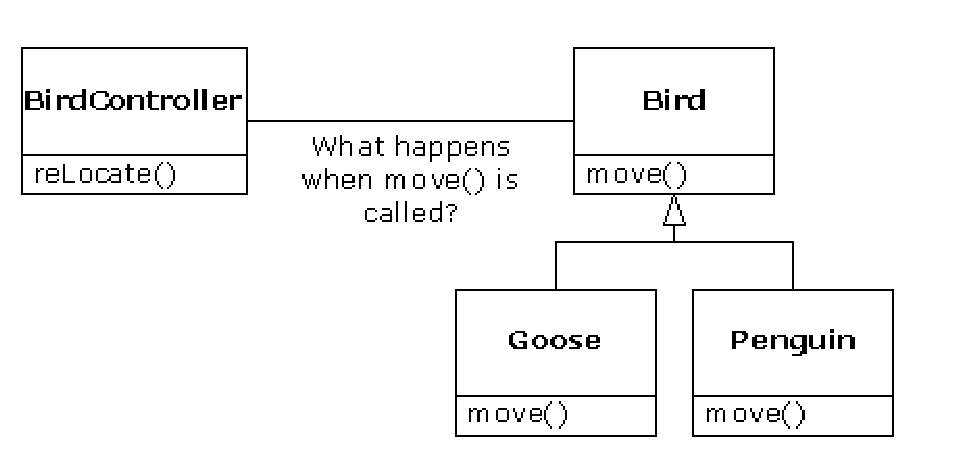
\includegraphics[scale=0.8]{eps/TIJ210.eps}
\end{figure}

這個問題的答案,是物件導向程式設計中最重要的訣竅所在:
編譯器無法以傳統方式來進行函式的叫用。由non-OOP 編譯器所產生的函式叫用,
會以所謂「前期繫結(early binding)」方式來呼叫函式。
這個名詞你過去可能從未聽聞,因為你從未想過能夠以其他方式來辦理。
運用這種方式, 編譯器對叫用動作產生出特定的函式名稱,而聯結器
(linker)再將此叫用動作決議(resolves)為「欲執行之程式碼的絕對位址」。
但是在 OOP 中,程式未到執行期是無法決定程式碼的位址的,
因此當我們將訊息發送給泛化物件 (generic object) 時,必須採用其他解決方案。

為了解決上述問題,物件導向程式語言採用所謂的「後期繫結(late
binding)」觀念。當你發送訊息給物件,
「應被喚起的程式碼」會一直到執行期才決定下來。編譯器還是有責任確定函式的存在,
並對引數 (arguments)、回傳值(return value)進行型別檢驗
(無法對此提供保證者,即所謂「弱型別(weakly typed)」語言),
但編譯器仍舊無法得知究竟會執行哪一段程式碼。

為了達到後期繫結,\marginpar{\fbox{46}} Java
使用一小段特殊程式碼來代替呼叫動作的絕對形式。
這一小段程式碼會透過物件內儲存的資訊來計算函式實體位址
(此一過程將於第七章詳述)。因此每個物件可因為這一小段程式碼的內容不同,
而有不同的行為。當你發送訊息至某個物件,該物件便知道如何反應。

在某些程式語言裡頭(例如C++),你得明確指出是否希望某個函式具備後期繫結的彈性。
這一類語言把所有 member functions 的繫結動作預設為 「非動態」。
這會引起諸多問題,所以Java 將所有member functions 預設為動態繫結
(後期繫結),你不需要加上任何關鍵字,就可以獲得多型 (polymorphism)的威力。

回頭想想「形狀」的例子。整個classes 族系(擁有一致介面的所有 classes)
在本章稍早已有圖示。為了說明多型(polymorphism)特性,我要撰寫一段程式碼,
並在程式碼中忽略型別(types)細節,僅和 base class 溝通。
這樣的程式碼和「型別特定資訊」之間已經解除耦合 (decoupled) 了,
撰寫起來格外簡單又容易理解。舉個例子,當新型別
「六邊形(Hexagon)」透過繼承機制加入classes 族系時,
處理舊型別的程式碼不需任何改變便可以處理新型別。也因此,
我們說這個程式是可擴充的(extensible)。

如果以Java 來撰寫函式(很快你就會學到如何撰寫):
\begin{verbatim}
void doStuff(Shape s) {
s.erase();
// ...
s.draw();
}
\end{verbatim}

上述函式可以和任何 Shape 交談,獨立於它所繪製或擦拭的任何特定物件型別。
如果我們在程式的其他地點用到了doStuff() 函式:
\begin{verbatim}
Circle c = new Circle();
Triangle t = new Triangle();
Line l = new Line();
doStuff(c);
doStuff(t);
doStuff(l);
\end{verbatim}

那麼\marginpar{\fbox{47}}當呼叫doStuff() 時,不論物件之實際型別為何,
都能夠運作無誤。 這是個令人感到驚奇的手法。再看看下面這行程式:
\begin{verbatim}
doStuff(c);
\end{verbatim}

此處當Circle 被傳入這個預期接收Shape 的函式時,究竟會發生什麼事呢?
由於Circle 是一種(is-a)Shape,所以它可被doStuff() 認可。亦即「doStuff()
可發送給Shape」的所有訊息,Circle 都可以接受,所以這麼做是完全安全且合邏輯的。

我們把「將derived class 視為其base class」的過程,稱為「向上轉型
(upcasting)」。cast 這個字的靈感來自於模型鑄造時的塑模動作,up
這個字則是因為繼承階層圖通常將base class 置於上端而將derived class
安排於下端,因此,轉型為一個base type,便是在繼承圖中向上移動,所以說是
upcasting。

\begin{figure}[htbp]
\centering
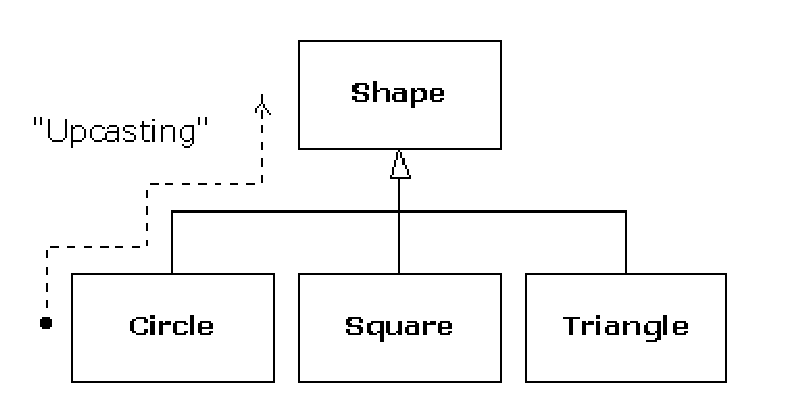
\includegraphics[scale=0.9]{eps/TIJ211.eps}
\end{figure}

物件導向程式一定會在程式某處做些upcasting 動作,
這正是你如何將自己從「執著於實際型別」救贖出來的關鍵。請看doStuff() 內的函式碼:
\begin{verbatim}
s.erase();
// ...
s.draw();
\end{verbatim}
注意,這裡並非表現出「如果你是Circle,請做這些事;如果你是
Square,請做那些事...」。如果撰寫那樣的碼,你得逐一檢查 Shape
物\marginpar{\fbox{48}}件的實際型別,那會帶來極大麻煩,因為每當加入新的
Shape type,你就得改變這段程式碼。這裡所表現的意思是「如果你是Shape,
我知道你自己可以erase(),可以draw(),請妥善進行,並小心細節處不要出錯。」

doStuff() 的內容實在令人感到神奇,不知怎麼地,事情竟然能夠自己搞定。
呼叫 Circle draw() 所執行的程式碼,和呼叫Square 或
Line 的 draw() 所執行的程式碼完全不同。當draw() 這個訊息發往不知所以的
Shape 時,竟會依據該Shape 的實際型別產生正確的行為。這真是神奇,
因為就如先前所說,當Java 編譯器編譯doStuff() 函式碼時,無法精確知道
doStuff() 所處理的型別究竟為何。所以你大概會預期,它呼叫的是
base class 的erase() 和draw(),而不是Circle、Square 或Line
的版本。多型(polymorphism)是整個神奇事件的幕後推手。
編譯器及執行期系統會處理相關細節,你只需知道這件事情會發生,
並知道如何透過它來進行設計,這就夠了。當你發送訊息給物件時,
即便動用了向上轉型 (upcasting),物件仍然會執行正確動作。

\subsection{抽象基礎類別與介面 \\(Abstract base classes and interfaces)}

通常在一個設計案中,你會希望base class 僅僅代表其derived class 的介面。
也就是說,你不會希望任何人產生base class 的實際物件,而只希望他們向上轉型至
base class - 這使得其介面可以派上用場。如果這確實是你的願望,可以使用關鍵字
abstract(抽象的)來標示某種class 是「抽象的」。如果有人試著為抽象類別產生物件,
編譯器會加以阻止。這是強迫某種特殊設計的好工具。

你也可以使用關鍵字 abstract 來描述「目前尚未實作完全」的函式,形成一種戳記
(stub),表示「衍生自此class 的所有型別,都有此一介面函式,
但它目前尚無實作內容」。抽象函式僅能存在於抽象 class 之中。當
class 被繼承,抽象函式必須被實作出來,否則新的 class 仍然是個抽象
class。「建立抽象函式」讓你得以將它置於介面之中,
無需被迫為該函式提供或許毫無意義的程式內容。


關鍵字 interface\marginpar{\fbox{49}}
(介面)又更進一步地發揮抽象概念,阻止任何一個函式被定義出來。
interface 是個常被用到而又十分方便的工具,
因為它提供了「介面和實作分離」的完美境界。此外,如果你想要,
你可以將多個介面組合在一起,不過你無法同時繼承多個一般的或抽象的 classes。
\section{物件的形貌與壽命 \\(Object landscapes and lifetimes)}
技術上來說,OOP 只談論抽象資料型別、繼承、多型等議題。
然而其他議題也可能同樣重要,本節剩餘篇幅涵蓋了這些議題。

一個極為重要的議題便是物件的生成(created)和毀滅(destroyed)。
物件的資料存於何處?它們的壽命如何控制?這裡有一些不同的處理哲學。
C++ 認為效率是最重要的議題,因此將抉擇留給程式設計者。想取得最好的執行速度?
沒問題,請將物件置於stack(這樣的物件又稱為automatic
變量或scoped 變量)或靜態儲存區中,於是程式撰寫時便決定了物件的儲存空間和壽命。
這種安排是把重點擺在儲存空間的配置與釋放的速度上。
某些情況下這樣的安排可能很有價值。不過這麼做卻也犧牲了彈性,
因為你必須在程式撰寫期間明確知道物件的數量、壽命、型別。
如果你企圖解決的是比較一般化的問題(例如電腦輔助設計、倉儲管理、飛航管制系統等),這種方式就過於受限了。

第二種方法是從一塊名為heap(堆積)的記憶體中動態產生物件。在這種方式之下,
除非等到執行期,否則你無法回答需要多少物件、壽命為何、 確切型別為何...等問題。
這些問題只有程式執行時方能給出答案。如果你要求新的物件,只需在必要時候從
heap 產生出來即可。由於執行期對儲存\marginpar{\fbox{50}}空間的管理方式是動態的,
所以從heap 配置空間所耗用的時間,遠大於從
stack 產生儲存空間所需的時間。是的,自stack 產生儲存空間,其動作通
常只是一個簡單的組合語言指令,將stack 指標往下移動;釋放時只要將
它往上移回即可。動態法有一個前提:適用於「物件比較複雜」的情況,
因此不論儲存空間的找尋或釋放時必要的額外負擔,都不致於對物件的產生造成重大衝擊。
動態法帶來的彈性,正是解決一般化程式問題不可或缺的根本。

Java 全然採用第二種方法\footnote{稍後你會看到,基本型別(primitive types)
是特例。}。
每當你想要產生物件,都得使用關鍵字 new 來動態產生物件的實體(instance)。

還有一個議題,就是物件的壽命。在那些「允許物件誕生於stack 內」的程式語言中,
編譯器會判斷物件應該存活多久,並可自動消滅之。但如果在 heap 之中生成物件,
編譯器對其壽命將一無所知。以C++ 為例,你得自行撰寫程式碼來摧毀物件。
因此如果不能正確做好此事,就會引發記憶體洩漏 (memory leaks),這幾乎是
C++ 程式的共通問題。Java 提供了所謂「垃圾回收器(garbage collectioncollector)」
機制,當物件不再被使用,會被自動察覺並消滅。垃圾回收器十分便利,
因為它可以減少你需要考量的因素,也減少你必須撰寫的程式碼數量。更重要的是,
垃圾回收器提供了更高階的保障,避免隱晦的記憶體洩漏問題發生
(這是許多 C++ 專案的痛處)。

本節的其餘篇幅,我們來看看諸多和物件壽命及其景貌相關的其他要素。


\subsection{群集器和迭代器 (Collections and iterators)}\marginpar{\fbox{51}}
如果你不知道你將動用多少個物件,或者不知道這些物件該存活多久,
才能夠解決某個問題,那麼你同樣無法知道該如何儲存這些物件。
如何才能夠知道該為這些物件準備多少空間呢?這其實永遠得不到答案,
因為這些資訊只有在執行期才能獲得。

相對於大多數物件導向設計問題而言,這個問題的解法似乎太過簡單:
產生另一種型別的物件。這個新型物件儲存著一些 reference,代表其他物件。
當然你可以使用array 完成相同的事情,大多數程式語言都提供 array。
不過這裡談的更多。這種新型物件通常被稱為容器(container),
有時也叫群集(collection)。由於Java 標準程式庫以不同的意義使用後一個術語,
本書決定採用「容器」一詞。這個新式物件會適當擴展自己的容量,
以便容納你置入的所有東西。你不需要知道將來會置入多少個物件於容器中,是的,
只要產生容器,它會自行料理細節。

幸運的是,好的 OOP 語言往往都會伴隨一組容器,做為套件的一部份。在 C++ 中,容器是
C++ 標準程式庫的一部份,有時候也稱為 Standard Template Library
(STL, 標準模板程式庫)。Object Pascal 在其視覺化元件庫
(Visual Component Library, VCL) 中亦提供了諸多容器。Smalltalk 提供的容器更完備。
Java 也在其標準程式庫中提供了許多容器。在某些程式庫中,
通用型容器能夠完善符合所有需求,其他程式庫(例如Java)則提供了諸般不同的容器,
符合各類需求。例如vector(向量,Java 稱之為 ArrayList)
為所有元素提供了一致性的存取方式,linked list(串列)
則提供任何位置上的元素安插動作。你應該挑選符合需求的容器。容器還可能包括:
sets(集合)、queues(佇列)、hash tables(雜湊表)、trees (樹狀結構)、stacks
(堆疊)等等。

所有容器都以相同的方式處理元素的置入和取出。通常它們都會提供元素安插函式,
以及元素取回函式。不過元素的取出動作較為複雜,
因為「只能進行單一選取動作」的函式實在是束縛過多,綁手綁腳。
如果你想同時操作或比較「一組」(而非一個)元素時,怎麼辦呢?

迭代器(iterator)\marginpar{\fbox{52}} 為此提供了解決之道。做為一個物件,
迭代器的作用就是用來選擇容器中的元素,並將這些元素呈現給迭代器使用者。身為一個
class,迭代器提供了某種抽象層級,
可將「容器實作細節」和「對容器進行存取動作之程式碼」分離開來。經由迭代器,
容器被抽象化為僅僅是一組序列 (sequence) 。迭代器讓你得以走訪整個序列,
無需煩惱底層結構究竟是 ArrayList 或 LinkedList 或 Stack 或其他。
這種彈性使我們可以輕易更動底層結構而不至於干擾應用程式碼。 Java 在版本 1.0 和
1.1 時代有個名為 Enumeration 的標準迭代器,用於所有容器類別之上。 Java 2
加入更完備的容器類別庫,其中包含名為 Iterator 的迭代器,它能用於老式
Enumeration 力所未逮的許多事情上面。

從設計觀點來看,你需要的其實只是一個可以被操作、用來解決問題的序列。
如果單單某個序列型別就可以滿足你的全部需求,實在沒有理由動用其他類型的序列。
不過,基於兩個理由,你還是得面臨容器的選擇。第一,
不同的容器提供了不同形式的介面和外在行為。stack 具備的介面與行為皆異於
queue,也和set、list 不同。
這些容器之間往往某一種會比另一種更能為你的問題提供彈性解答。第二,
不同的容器在某些操作上有著不同的效率,最佳例子便是 ArrayList 和 LinkedList。
這兩種序列具備完全相同的介面與外在行為,但在某些操作上所耗費的代價,
卻有截然不同的表現。對 ArrayList 進行隨機存取,可以在常數時間 (constant-time)
完成;不論你所選擇的元素為何,所需時間都相同。但是對 LinkedList
而言,「隨機選取某一元素」的動作需得在串列上行進,愈靠近串列尾端,
花費的時間愈久。另一方面,如果你將元素安插至序列中央位置,對 LinkedList
來說花費的代價明顯少於 ArrayList。不同動作的效率高下,
完全取決於序列的底層結構。在設計階段,也許一開始你採用
LinkedList,然後為了調校系統效能,轉而採用ArrayList。迭代器所帶來的抽象化,
使我們在進行諸如此類的轉換時,得以將衝擊降至最低。

最後,\marginpar{\fbox{53}}請你牢記,容器只是個可以將物件放入的儲藏櫃。
如果這個儲藏櫃可以解決你的全部需求,那麼它的實作方式就無關緊要
(對大多數類型的物件而言,這是基本觀念)。如果你所處的開發環境,
有著其他因素所引起的額外負擔,那麼,介於 ArrayList 和 LinkedList
之間的差別可能無關痛癢。你也許只需要一種序列型別。
你甚至可以想像有一個完美的容器抽象化機制,可以根據被運用的方式,
動態改變其底層實作方式。
\subsection{單根繼承體系 (The singly rooted hierarchy)}
OOP 中有個議題,在C++ 面世之後變得格外受人注目:所有classes
最終是否都繼承自單一的base class 呢?Java(以及大多數OOP 程式語言)
的答案是 yes,而且這個終極的 base class 名為 Object。
事實證明,單根繼承體系可以帶來許多好處。

單根繼承體系中的所有物件都有共通介面,所以最終它們都屬於相同的
type。在另一種(C++ 所提供的)設計中,你無法確保所有物件都隸屬同一個基本型別。
從回溯相容的觀點來看,這麼做比較符合C 模型,並且比較不受限制。
但是當你想要進行完全的物件導向程式設計時,就得自行打造自己的繼承體系,
以便提供某種便利性,而這種便利性在其他語言上卻是內建的。
你的程式庫內部可能會有一些不相容介面,你得額外花費力氣將新介面融入你的設計之中
(天啊,面對的可能是多重繼承)。C++ 是否值得為了前述的額外「彈性」這麼做呢?
如果你需要的話 - 也許你在 C 語言上面投資頗多 - 這麼做就有價值。
但如果你剛自起跑線出發,Java 這種方式通常會帶給你更大的生產力。

單根繼承體系(一如Java 所提供)保證所有物件都擁有某些功能。在整個系統裡,
你因此知道可以在每個物件身上執行某些基本操作。單根繼承體系再加上
「在heap 之中產生所有物件」,大大簡化了引數傳遞動作(這也是
C++裡頭十分複雜的問題之一)。

單根繼承體系也使垃圾回收器\marginpar{\fbox{54}} (內建於Java) 的實現更加容易。
所有必備功能都可安置於base class 身上,
然後垃圾回收器便可發送適當訊息給系統中的每個物件。
如果缺乏「單根繼承體系」及「完全透過 reference 來操作物件」的系統特性,
垃圾回收器的實作就會十分困難。

由於所有物件都保證會有執行期型別資訊(run-time type information,
RTTI),所以你必不會因為無法判斷物件的確切型別而陷入動彈不得的僵局。
對於異常處理(exception handling)之類的系統級操作行為而言,這一點格外重要,
並且也能為程式設計帶來更佳彈性。
\subsection[群集類別庫,及其易用性支援]{群集類別庫,及其易用性支援 \\
Collection libraries and support for easy collection use}
容器是一種常常被使用的工具,所以將容器程式庫製成內建形式,是很有意義的事情。
這麼一來你就可以直接使用現成的容器,將它套入你的應用程式中。
Java 提供了這樣的程式庫,而且幾乎可以滿足所有需求。
\subsubsection{向下轉型 vs.模版/泛型 (Downcasting vs. templates/generics)}
為了重複運用容器,我們會以Java 中的某個通用型別(也就是Object)
為對象,進行儲存工作。單根繼承體系意謂「萬物皆為Object」,因此,
如果容器可以裝納 Objects,也就可以儲存任何物件。這使得容器很容易被重複運用。

欲使用這樣的容器,只需將object reference 加入即可,稍後可以將它們取回。
由於容器僅容納 Objects,所以當你將物件的reference 加入容器時,
會向上轉型為 Object,因而遺失自己的精確身份。當你將它取回,你所得到的僅僅是個
Object reference,而非你所置入之物件的確切型別。現在,
該透過怎樣的方式將它變回先前那個具備實用介面的物件呢?

在這裡,轉型動作再度派上用場。但這一次並非是在繼承體系中向上轉型為更通用的型別,
而是向下轉型為更特定的型別。這種轉型動作稱為向下轉型
(downcasting) 。你已經知道, 向上轉型( 例如Circle 轉為\marginpar{\fbox{55}}
Shape)十分安全。但由於你無法得知某個Object 是否為Circle 或
Shape,所以除非你確切知道你所處理的是什麼,否則向下轉型幾乎是不安全的。

不過向下轉型也非全然危險,因為如果向下轉型至錯誤的型別,你會得到所謂「異常
(exception)」的執行期錯誤,稍後我會簡短介紹什麼是異常。但即便有此機制,
從容器中取出object references 時,
你還是需要某種方式來記住這些物件究竟是什麼型別,才能夠放心進行向下轉型。

向下轉型及執行期檢驗動作,都會耗費額外的程式執行時間,以及程式設計者的心力。
何不建立起「知道自己所儲存之物件隸屬何種型別」的容器,
藉以降低向下轉型的需求及可能導致的錯誤呢?解決之道就是所謂的
「參數化型別(parameterized types)」,這是一種由編譯器自動為我們量身訂製的
classes,作用於特定型別之上。舉個例子,如果使用這類參數化容器,
編譯器便可訂製此一容器,使它只能接受(及取出)Shapes。

參數化型別(parameterized types)是C++ 極為重要的組成,部份原因是
C++ 缺乏單根繼承體系。在C++ 中,實現參數化型別的關鍵字是
template。Java 目前並沒有參數化型別,因為單根繼承體系已經可以涵蓋
「參數化型別」的功能。不過目前有一份相關提案,其中採用和C++
template 極為相似的語法(譯註:JSR14,目前已實現於JDK1.4 和
GJ 身上,見www.jjhou.com/javatwo-2002.htm)。
\subsection[管家面臨的兩難:誰該負責清理?]{管家面臨的兩難:誰該負責清理? \\
The housekeeping dilemma: who should clean up?}
每個物件為了生存,都需要動用資源,尤其是記憶體。當物件不再需要記憶體,
就該加以清除,使資源可被釋放、可再被使用。在相對簡單的程式設計環境中,
清理物件似乎不是什麼困難的問題:首先產生物件,然後使用之,
最後它就應該被摧毀。這不難,但你可能遭遇更為複雜的情況。

舉個例子,假設你正在設計機場航空交通管制系統
(同樣的模式在倉儲貨物管理、錄影帶出租系統、寵物寄宿店一樣適用)。
一開始問題似乎很簡\marginpar{\fbox{56}}單:做出一個容器,用來置放飛機,
然後產生新飛機,然後把每一架位於飛航管制區的飛機放到容器之中。
一旦飛機飛離該區域,刪去對應的物件,即是完成了清理動作。

但你或許還有其他系統,記錄著飛機的相關資訊;
或許這些資料目前不會馬上為主控功能所用。
它可能記錄所有即將離開機場之小型飛機的飛行計畫。所以你會有第二個容器,
用來儲存所有小型飛機;每當你產生一個小飛機物件,
同時也把它置於第二容器中。然後,在程式閒置時間(idle time)以一個背景行程
(background process)操作第二容器內的物件。

現在問題更加困難了:何時才是消滅這些物件的適當時機?當你用完某個物件之後,
系統中的某部份還有可能再使用它。此類問題會發生在其他許多情境之中,
在那些「你必須明確刪除物件」的系統中,這件事情顯得格外複雜。

Java 的垃圾回收器被設計用來處理「釋放記憶體時可能會有的種種問題」
(其中並未包含物件清理動作的其他面向問題)。垃圾回收器會「知道」
物件何時不再被使用,然後自動釋放該物件所用的記憶體。這種方式合併了
「單根繼承體系」和「完全從heap 配置記憶體」兩大特性,使得透過
Java 進行程式設計的過程遠較透過C++ 單純。只需做極少量決策,
只有極少的障礙需要克服。

\subsubsection{垃圾回收器vs.效率與彈性 \\
Garbage collectors vs. efficiency and flexibility}
如果這麼做沒有任何瑕疵,為什麼C++ 不率先採行?是的,當然,
你得為程式設計上的便利付出代價,這個代價就是執行期的額外負擔。一如先前所述,在
C++ 中,你可以選擇在stack 上生成物件,它們會被自動清除
(但不具備彈性,無法在執行期依需要而動態產生)。在stack
上生成\marginpar{\fbox{57}}物件,
對儲存空間的配置和釋放來說幾乎是最有效率的方式。在 heap 上生成物件,
代價可就高昂多了。即使完全繼承同一個 base class,完全以多型
(polymorphic)方式來處理函式呼叫,還是需要付出少量代價。
垃圾回收器之所以特別形成癥結,問題在於你永遠不知道垃圾回收動作何時開始、
持續多久。這意謂Java 程式的執行速率會有不一致的現象,因此無法應用於某些情況下,
例如在極重視程式執行速率的場合。此類程式通常稱為即時
(real time)程式 -  雖然並非所有的即時程式設計問題都如此嚴峻。

C++ 的開創者努力爭取 C 程式員的支持,而且成果豐碩,
因此不希望加入任何影響速度的功能,也不期望在那些「程式員可能會選擇
C 的場合」因為 C++ 所引進的新功能轉而採用 C++。這個目標達到了,
但也使得以 C++ 進行設計時需付出「高複雜度」的代價。相對於 C++,
Java 單純許多,但這種單純換來的便是效率上的折損,有時也會失去適用性。然而,
對於解決大多數程式問題而言,Java 是較好的選擇。

\section[異常處理:面對錯誤的發生]{異常處理:面對錯誤的發生 \\
Exception handling: dealing with errors}
自從天地間有了第一個程式語言,錯誤的處理始終都是最困難的問題之一。
因為良好的錯誤處理系統很難設計,所以許多程式語言乾脆直接略去這個議題,
將它留給程式庫設計者,由後者提供「可用於許多情況,但是並非完全徹底」的方法,
或甚至完全忽略這個議題。大多數錯誤處理系統的問題在於,
它們十分依賴程式員自身的警覺性,而非語言本身的法制性。
如果程式員本身不夠警覺 - 通常是因為專案太趕 - 這些系統便容易被忽略。

「異常處理機制」將錯誤處理問題直接內嵌於程式語言中,
有時甚至直接內嵌於作業系統中。所謂異常(exception)是一種物件,
可在錯誤發生點\marginpar{\fbox{58}}被擲出(throw),並在適當的處理程序中被捕捉
(catch),藉以處理特定類型的錯誤。當錯誤發生,
異常處理機制會採取一條截然不同的執行路徑。
也正因為如此,所以它不會干擾程式碼的正常執行。這使得程式碼的撰寫更加單純,
因為你不需要被迫定時檢查錯誤。此外,被擲出的異常、 函式回傳的錯誤值、
函式為表示錯誤發生而設定的旗標值,三者之間有著本質上的差異 -
後二者都可以被有意忽略,異常則無法被忽略,保證一定會在某處被處理。最後一點:
異常為「錯誤情境的確實回復」提供了一種可行方案,是的,不再只能選擇退出
(那是一種逃避),如今你可以校正事情,回復程式的執行,
這種表現是穩健而強固的程式的特質。

Java 的異常處理機制在眾多程式語言中格外引人注目,因為
Java 一開始就將異常處理機制內嵌進來,強迫你使用。
如果你沒有撰寫可適當處理異常的程式碼,便會發生編譯錯誤。
這種一致的態度使得錯誤處理更加容易。

雖然物件導向程式語言常以一個物件表現一個異常(exception),
但異常處理機制並非物件導向的特性。是的,異常處理機制在物件導向語言出現之前,
存在久矣。
\section{多執行緒 ( Multithreading)}
電腦程式設計有一個很基礎的觀念,那就是必須能夠同時處理多個工作
(task)。許多設計上的問題,需得程式停下手頭的工作,處理一些其他事情,
再返回主行程(main process)。辦法很多,早期程式員透過對機器的低階認知,
撰寫中斷服務常式(interrupt service routines),透過硬體中斷的觸發,
暫停主行程的執行。雖然這麼做沒有問題,但這種作法難度較高,也不具可攜性。

有時候,\marginpar{\fbox{59}} 在處理「時間因素極為關鍵」的工作(task)時,
中斷的使用是必要的。但還有其他為數不少的問題,
只需將問題切割為多個可獨立執行的片段,便能夠讓整個程式更具反應力。
這些「可獨立執行的片段」便是所謂的執行緒( threads ) ,
而上述這種觀念便被稱為「多緒」 (multithreading)。
最常見的例子便是使用者介面的運作了,透過執行緒的使用,
雖然還有某些處理動作正在電腦中進行,使用者仍然可以按下按鈕,不受阻礙。

通常,執行緒只是一種用來「配置單一處理器執行時間」的機制。
但如果作業系統支援多處理器的話,不同的執行緒便可以被指派至不同的處理器執行,
真正做到並行(parallel)執行。在程式語言這個層次上提供多執行緒,
所能達到的便利之一便是,讓程式設計者無需考量實際機器上究竟存在多少個處理器。
程式只是邏輯上被劃分為多個執行緒,如果機器擁有多個處理器,不需特別的調整,
程式就能夠執行得快一些。

這使得執行緒聽起頗為單純,但當發生資源共享時,卻會出現隱約的問題。
倘若多個並行的執行緒共用同一份資源,就會引發問題。舉例來說, 兩個行程
(processes)無法同時送出資訊至單一印表機。為了解決這個問題,某些可被共享的資源
(例如印表機),必須在使用時加以鎖定。因此整個過程是:執行緒鎖住某資源、
完成自己的工作、解除鎖定讓其他行程有權力使用該資源。

Java 在程式語言中內建了執行緒功能,讓此一複雜課題變得單純。
由於執行緒功能是在物件層次上提供,因此一個執行緒便以一個物件來表示。
Java 也提供有限的資源鎖定功能,可以鎖定任何物件所用的記憶體
(也算是某種形式的資源鎖定),使得同一時間內只有一個執行緒可使用這個物件。
透過關鍵字synchronized 便可達到此一目的。其他型態的資源就必須靠程式員自行鎖定,
通常的作法是產生一個物件,代表欲鎖定的資源;
所有執行緒在存取這份資源之前都必須先加以檢驗。

\section{永續性 (Persistence)} \marginpar{\fbox{60}}
物件生成之後,只要你還需要它,它就會持續存在。但是一旦程式結束,
它就不再有生存環境了。如果物件可以在程式非執行狀態下依舊存在、依舊保有其資訊,
那麼在許多應用中將大有幫助。因為當程式重新啟動,物件便又能夠復活,
而且仍然具備上次執行時的狀態。當然,你可以簡單地將資料寫到檔案或資料庫,
進而達到這個效果。但是在「萬事萬物皆物件」的精神下,如果能夠將物件宣告為永續的
(persistent),而且由語言系統自動為你處理所有相關細節,不就太好了嗎?

Java 提供所謂的「輕量級永續性(light weight persistence)」,
讓你可以很輕鬆地將物件儲存於磁碟,並於日後取回。稱「輕量級」的原因是,
你還是得自己呼叫儲存、取回動作。除此之外,JavaSpaces(第十五章敘述)
還提供另一種永續儲存功能。未來版本可能還會提供更完整的支援。
\section{Java 與Internet(網際網、互聯網)}
如果Java 不過是程式語言芸芸眾生中的一個,你可能會問,為什麼它如此重要?
為什麼會被宣傳為電腦程式設計革命性的一大步。從傳統程式設計的觀點來看,
答案並不那麼明顯。雖然Java 在解決傳統的個別程式設計問題上非常有用,
但更重要的是,它能夠解決World Wide Web(全球資訊網,萬維網)上的程式設計問題。
\subsection{Web 是什麼?}
Web 一詞,就像其他諸如surfing(網絡衝浪)、presence、home pages
(首頁)等詞彙一樣,乍見之下可能難以理解。對於Internet 這波狂潮,
愈來愈強的反向力量在質問著,這波其勢難擋的變動,經濟價值和結果究竟為何。
如果我們回頭審視其真實面貌,應該會大有幫助。要這麼做,就得先從所謂的「主從
(client/server)」系統開始了解。
這個系統正是電算技術中另一個令人充滿諸多困惑的東西。

\subsubsection{主從式電算技術 (Client/Server computing)} \marginpar{\fbox{61}}
主從式系統的核心概念是,系統中存在一個集中的資訊貯存所,貯存某種形式的資料,
通常位於資料庫中。你想要將這些資訊依據需求,傳佈給某些人或某些機器。
主從概念的關鍵核心便在於,資訊貯存的位置集中於一點。因此每當該點的資訊改變,
變動結果便會傳播至資訊使用者手上。綜合言之,資訊貯存處是一套軟體系統,
能將資訊傳播出去,而資訊和軟體系統所在的機器(可能是單部機器,可能是多部機器)
便稱之為伺服器 (server)。位於遠端機器上、和伺服器溝通以便擷取資訊、處理資訊、
顯示資訊的軟體系統,便稱為用戶端(client)。

主從式計算的基本觀念並不複雜。問題出在你只有單一伺服器,卻必須同時服務多個用戶。
一般而言這會動用所謂的資料庫管理系統,讓設計者得以安排「資料置於表格 (table)
中的佈局方式」,藉以取得最佳使用效果。除此之外,
系統通常也允許用戶增加新的資訊至伺服器。
這意謂你必須確保某個用戶的新資料不會覆蓋另一個用戶的資料,
並確保資料在加入資料庫的過程中不會遺失, 此即所謂的交易處理機制( transaction
processing)。一旦用戶端軟體有所改變,它們必須被設置、被除錯、
然後被安裝於用戶端機器上。整個過程可能超乎你想像的複雜與費力。
如果想同時支援多種不同類型的電腦或作業系統,事情更是格外麻煩。
最後還有一個重要課題:效率。是的,
可能有數以百計的用戶同時向伺服器發出請求,因此即便是一點小小延遲,
都可能帶來重大影響。為了降低延遲,程式員必須努力分散欲處理的工作,
通常是分散至用戶端機器,但有時候會使用所謂的中介軟體 (middleware),
分散至伺服端的其他機器。中介軟體也被用來改善系統的可維護性(maintainability)。

「將資訊分散至多處」的這個單純想法,實作上卻有極多層次的複雜度,
整個問題簡直是棘手得令人絕望。然而主從運算幾乎主宰了半數的程式設計活動。
從訂貨、信用卡交易到各種形式- 股市、科學、政府、個人 -\marginpar{\fbox{62}}
的資料傳佈。過去以來的路線是,每面對一個新問題,就發明一個新的解決方法。
這些方法都很難開發,很難使用,使用者必須一次又一次學習新的介面。
主從架構下的問題需要一個全面性的解決。
\subsubsection{Web 就是一個巨型伺服器 (The Web as a giant server)}
整個Web 體系,實際上就是個巨大的主從系統。更糟的是,
所有的伺服器與用戶端同時共存於同一個網絡中。不過你沒有必要知道這件事,
雖然你可能會為了搜尋想要的伺服器而遍尋全世界,
但同一時間你只要考慮單一伺服器的連接與互動就好了。

剛開始只是很單純的單向過程:向伺服器提出請求,然後伺服器回傳一份檔案,
機器上所執行的瀏覽器(一種用戶端軟體)便根據本機(local machine)
上的格式來解讀這份檔案。但是很快地,人們開始進行更多嘗試,
不單從伺服器擷取檔案,還希望擁有完整的主從架構能力,
讓用戶端也能將資訊回饋至伺服端,例如在伺服器上進行資料庫的搜尋、
將新資訊加入伺服端、下訂單(所需的安全性比早先系統所能提供的還要高)等等。
這樣的歷史變革,是我們可以從Web 的發展過程中觀察到的。

Web 瀏覽器的概念更是向前跨了一大步:同一份資訊可以不需任何改變,
便顯示於各種類型的電腦上。但瀏覽器仍然過於原始,
很快便因為加諸其上的種種需求而陷入困境。是的,瀏覽器缺乏完備的互動能力,
不論你想做什麼事情,幾乎都得面對「將資訊送回伺服器去處理」的問題。
也許花費了幾秒鐘、甚至幾分鐘之後,才發現你所輸入的資料拼字錯誤。
這是因為瀏覽器只是一個觀看資料的工具,無法執行任何即便是最簡單的計算工作。
從另一個角度看,這樣倒也安全,
因為這樣就無法在你的本機上執行任何可能帶有臭蟲或病毒的程式。 

數種不同的方法可以解決這個問題。首先是改善圖形標準規格,
因而得以在瀏覽器中撥放較佳的動畫和視訊。
其餘問題必須透過「在瀏覽器上執行\marginpar{\fbox{63}}程式」的方式加以解決。
此即所謂「用戶端程式開發( client-side programming)」。
\subsection{用戶端程式開發 \\(Client-side programming)}
Web 最初的「伺服器-瀏覽器」設計方式,可提供互動性內容,
但這種互動完全由伺服器提供。伺服器產生靜態的頁面內容,瀏覽器簡單地加以解讀,
然後顯示。基本的HTML 包含有資料收集機制:文字輸入方塊(textentry boxes)、
核取方鈕(check boxes)、選取圓鈕(radio boxes)、列式清單(lists)、下拉式清單
(drop-down lists)等等。此外還包括按鈕 (button):可用於表單 (form)
資料的清除或提交(submit,傳給伺服器)。這種提交動作是透過任何一部
Web 伺服器都會提供的 CGI (Common Gateway Interface,共通閘道介面)
達成。提交內容會告訴 CGI 要做些什麼工作。
最常見的動作便是執行伺服器上某個目錄底下的某個程式,該目錄通常被命名為
``cgi-bin''。 (按下Web 頁面上的按鈕後,如果你觀察瀏覽器上方的位址視窗,
有時候便會看到 ``cgi-bin'' 字樣,後面跟著一大堆冗長不知所云的東西。)
幾乎所有程式語言都可用來撰寫這種類型的程式,Perl 是最常見的選擇,
因為它被設計用來處理文字,而且是解譯式語言,
因此無論伺服器所使用的處理器以及所安裝的作業系統是什麼,Perl 都可以安裝在上面。

今天,許多頗具影響力的Web 站台,完全以CGI 打造。
事實上你幾乎可以用它來達成所有目的。但是以 CGI 程式建構的 Web
站台可能很快會變得過於複雜而難以維護,並衍生「回應時間過長」的問題。
CGI 程式的回應時間和傳送資料量的多寡有關,
也和伺服器的負載以及網絡的擁擠程度有關。而且
CGI 程式的初始化動作先天上就比較慢。Web 初始設計者並沒有預見到,網絡頻寬
(bandwidth)是如此快速地被人們所發展出來的眾多應用程式耗盡。
因此任何形式的動態繪圖動作幾乎都不可能,因為得先產生一個個
GIF 檔案,再一個個從伺服端搬至用戶端。此外你一定也處理過 「驗證表單資料」
之類的簡單事情:你在某個頁面上按下 ``submit'' (提交) 鈕,資料便回送至伺服器,
然後伺服器執行某個 CGI 程式;這個程式\marginpar{\fbox{64}}查覺輸入資料的錯誤,
產生一份HTML 頁面通知你有誤,並將此頁面回傳給你;
於是你回到前一頁面,再試一次。這樣不僅十分緩慢,也不優雅。

這個問題的救星就是用戶端程式開發(client-side programming)。大多數執行
Web 瀏覽器的機器,其實都威力十足,可堪執行龐大的工作。在原始的靜態
HTML 方式下,這些機器只是杵在那兒等著伺服器送來下一個頁面。
「用戶端程式開發」所指的,便是利用Web 瀏覽器來執行某些它能夠執行的工作,
讓網站使用者覺得運行更迅速,操作介面更具互動性。

用戶端程式開發的問題在於,它和一般的程式開發極不相同。參數幾乎相同,
平台卻有差異:Web 瀏覽器就像一個功能受限的作業系統。當然,最後你還是得寫程式,
而且還是得處理那些令人頭暈眼花的問題,並以用戶端程式開發方式來完成解法。
這一節的剩餘部份,我便概觀性地討論用戶端程式開發中的諸般問題和解法。
\subsubsection{Plug-ins}
用戶端程式開發所跨出的一大步,便是發展所謂的 ``plug-in'' 。
透過這種作法,程式員得以下載一小段程式碼來為瀏覽器加入新功能。
那一小段程式碼會將自己安插到瀏覽器的適當位置。它會告訴瀏覽器:從現在開始,
你可以執行這種新功能。於是某些快速、具威力的功能便可透過 plug-in 加到瀏覽器上。
你只需下載 plug-in 一次就好。撰寫 plug-in 並不是件輕鬆的事,
也不是為特定網站而做的事。對用戶端程式開發而言,
plug-in 的價值在於它讓專家級程式員發展新形語言,並將該語言加至瀏覽器中,
而不須經過瀏覽器製造商的許可。因此,plug-in 提供了所謂的後門
(back door),藉以加入新的用戶端程式語言。當然啦,並非所有的用戶端程式語言皆以
plug-in 實作。


\subsubsection{Scripting(描述式、劇本式)語言}\marginpar{\fbox{65}}
Plug-in 帶來了script 語言的蓬勃發展。透過script 語言,
你可以將用戶端程式的原始碼直接內嵌於HTML 頁面中。一旦HTML 頁面被顯示,
負責解譯該語言的plug-in 便會被自動喚起。script 語言先天上比較容易理解,
而且它們只是HTML 頁面內的部份文字, 所以當伺服器收到請求
(request)而欲產生HTML 頁面內容時,可以很快加以載入。犧牲的是你的程式碼的隱密性。
不過通常我們不會使用script 語言做過於複雜的事情,所以隱密性的問題不算太嚴重。

這也點出了script 語言的缺點:只能在Web 瀏覽器中拿來解決特定型態的問題,
更明確地說是指用來建立更豐富、更具互動性的圖形使用介面
(GUIs)。script 語言的確可能解決用戶端程式開發過程中遭遇的百分之八十問題。
如果你的問題恰恰落在這百分之八十之中,script 語言可為你提供簡單快速的開發過程。
在考慮使用諸如Java 或ActiveX 之類更複雜的解法之前,或許你應該先考慮script 語言。

最常被討論的瀏覽器script 語言包括:JavaScript(和Java 毫無關連;
其命名只是為了搭上Java 浪潮而已)、VBScript(程式風貌和Visual Basic 相彷)、Tcl/Tk
(最受歡迎的跨平台GUI 程式設計語言)。還有一些 script 語言不在此列,
有一些正在發展之中。 

JavaScript 或許是其中最被廣泛支援的一種。Netscape Navigator 和微軟的
Internet Explorer(IE)都提供對它的內建支援。此外,比起其他瀏覽器語言,市面上的
JavaScript 書藉或許是最多的。有許多自動化工具可以使用JavaScript 自動產生頁面。
不過如果你已經對 Visual Basic 或 Tcl/Tk 駕輕就熟,
熟練地運用它們應該會比學習另一個新語言更具生產力,
因為你可以將全部心力集中於解決 Web 相關問題。

\subsubsection{Java} \marginpar{\fbox{66}}
如果script 語言可以解決用戶端程式開發問題中的百分之八十,其他的百分之二十
(那些真正很難的東西)該怎麼辦?現今最受歡迎的解決方案便是 Java。
不只因為它是個威力十足的語言,內建了安全功能、跨平台能力、
提供易於進行國際化動作的工具,而且更重要的是,Java
持續擴充其語言功能和其程式庫,得以優雅地處理傳統語言中諸多未能處理好的問題,
像是多緒、資料庫存取、網絡程式開發、分佈式計算。Java 係透過所謂的
applet 來進行用戶端程式開發。

所謂applet 是個小程式,只能執行於Web 瀏覽器上。做為Web 頁面中的一部份,
applet 會被自動下載(就像頁面中的圖形會被自動下載一樣)。
applet 被激化(activated)之後便開始執行,這是它優雅的地方之一 -
當使用者需要用戶端軟體時,便能夠自動將用戶端軟體從伺服器分發出去,
不需事先安裝。使用者絕對可以取得最新版本的用戶端軟體,不會安裝錯誤,
也不需要困難的安裝過程。由於Java 的這種設計,程式員只需發展單一程式,
該程式便能夠自動運作於所有電腦之上 -
只要這些電腦裝有「內建Java 解譯器」的瀏覽器即可(大多數機器都如此)。由於
Java 是個發展完備的語言,所以在將請求送往伺服器之前和之後,
你都可以盡情地在用戶端工作。例如你不必先透過網絡送出請求表單
(form),而後才發現所填的日期或參數錯誤。用戶端的電腦也可以快速繪出資料,
不必等待伺服器完成圖形繪製後才將圖形傳回。
你所獲得的不僅是高速度和高回應能力,也可以降低網絡流量和伺服器負載,
不至於拖累整個Internet 的運作速度。

Java 凌駕於script 語言之上的另一個優點就是,它是編譯式語言,
所以用戶端無法看到原始碼。雖然不需花太多力氣就可以對
Java applet 進行反譯動作,但程式碼的隱藏通常不是什麼重要課題。此外,
還有兩個重要因素。一如稍後所見,編譯過的 Java applet 可以由多個模組構成,
必須引發\marginpar{\fbox{67}}多次對伺服器的存取動作
(hits)才可以下載這些模組。(在Java 1.1 以及更新版本中,透過 Java 保存檔 -
所謂 JAR - 使得所有必要模組都能夠以壓縮形式包裝起來,
因此下載單一檔案便可取得所有模組。)script 程式只需以文字形式整合到
Web 頁面內即可(通常比較小,也減低對伺服器的存取),這對
Web 站台的回應速度很重要。另一個因素是極為重要的「學習曲線」。
不論你過去所學為何,Java 都不是個容易學習的語言。如果你是 Visual Basic 程式員,
那麼投向 VBScript 可能是你的最快解決方案,
它或許可以解決大多數普通的主從式架構問題,這些問題很難拿來印證
Java 的學習。如果你過去對 script 語言已有經驗,那麼付諸
Java 之前,先看看 JavaScript 或VBScript 會對你大有幫助,
因為它們可能更容易符合你的需求,而且使你更具生產力。
\subsubsection{ActiveX}
就某種程度而言,Microsoft ActiveX 和Java 比起來雖然骨子裡是完全不同的技術,
卻足堪與Java 競爭。ActiveX 原先僅用於Windows 系統上,但透過獨立的聯合性組織,
其跨平台能力正在成長。ActiveX 主張,如果你的程式只連接於自身所屬的環境,
那麼此程式便可直接內含於Web 頁面內, 並在支援 ActiveX 的瀏覽器上執行 - IE
直接支援ActiveX,Netscape 則需透過 plug-in 才能辦到。因此 ActiveX
並不侷限於特定的程式語言。舉個例子,如果你曾使用C++、Visual Basic、
Borland Delphi 等語言,在 Windows 平台上進行程式開發,
那麼幾乎不需改變任何程式設計知識,就可以產生 ActiveX 組件
(components)。ActiveX 也讓你得以移轉舊有程式碼至 Web 頁面中。
\subsubsection{安全性Security}
「自動透過Internet 下載程式並執行」聽起來簡直就是病毒作者的夢土。
ActiveX 特別帶起用戶端程式開發中關於安全性的議題。當你點擊某個
Web 頁面,可能會自動下載許多東西:GIF 檔案、script 程式碼、編譯過的
Java 程式碼、ActiveX 組件...。某些東西可能是良性的,例如GIF 檔就不會造成傷害,
script 語言能做的事情通常也都十分有限。Java 的設計理念中,也將
applet 的執行侷限於受到安全保護的砂盒(sandbox)內。
在\marginpar{\fbox{68}}砂盒裡頭,applet 無法對磁碟寫入資料,
也無法存取砂盒外的記憶體內容(譯註:砂盒是西方小孩普遍的玩具,
砂子只能在砂盒裡頭,不能溢出)

ActiveX 剛好位於光譜的另一端。ActiveX 程式開發就和一般的Windows
程式設計一樣,百無禁忌。如果你點擊了某頁面,因而下載了某個ActiveX
組件,此一組件便有可能破壞磁碟中的檔案。這是當然啦,只要你所載入的程式不受限於
Web 瀏覽器,便可以玩出相同的戲碼。來自電子佈告欄系統
(BBSs)的病毒,長久以來一直都是嚴重的問題,Internet 無遠弗屆的速度,
更強化了這個問題。

所謂「數位簽證(digital signatures)」似乎是解答所在。透過數位簽證,
我們可以檢驗程式作者究竟是誰。這個方法著眼於病毒的運作方式 -
病毒作者永遠是匿名的,如果能夠消除匿名行為,那麼每個人都必須為自己的行為負責。
乍看之下不錯,因為這麼做可以讓程式更加實用。
但我懷疑這麼做是否真能消除所有的惡意禍害。而且如果某個程式有臭蟲,
雖非故意造成破壞,仍然會導致問題發生。

透過砂盒(sandbox)的作法,Java 可以避免上述問題發生。存於本機
Web 瀏覽器之中的Java 解譯器(intepreter),在載入applet 的同時便檢驗
applet 是否含有不適宜的指令。因此applet 無法將檔案寫入磁碟,也無法刪除檔案
(而這些正是病毒的生存方式與為害方式)。applet 通常被視為安全,
而「安全」正是可靠的主從系統的支柱。Java 語言中任何可能滋生病毒的缺點,
都會被迅速修正。(瀏覽器軟體會強制施行這些安全限制,
某些瀏覽器甚至允許你選擇不同的安全等級,藉以提供不同等級的系統存取能力。
譯註:不僅瀏覽器可以這麼做,所有Java 程式都可以透過自訂
SecurityManager 的安全策略而辦到。)

你可能會質疑這個方法太過嚴苛,因為這樣就無法將檔案寫入本機磁碟。
舉個例子,你可能會想建立本機資料庫,或是將檔案儲存起來,留待離線時使用。
然而,即便最初的夢想是要讓每個人最終都可以在線上進行所有重要工作,
但大家馬上了解到這可能不切實際(直到有朝一日,
低成本的網絡設備可以滿足大部份使用者的需求)。簽證過的applet 可以回應你的質疑。
「公開金鑰加密」(public-key encryption)可以讓我們檢驗
applet\marginpar{\fbox{69}}是否真的出自它所宣稱的來源。雖然簽證過的
applet 仍然可能毀掉你的磁碟,但你現在可以相信
applet 的作者擔保他們不會進行惡意動作。Java 為數位簽證提供了完整的架構,
所以你還是可以在必要的時候讓applet 踏出砂盒的牢籠。

數位簽證遺漏了一個重要問題,那就是人們在Internet 上的行動速度。
如果你下載某個有問題的程式,而且該程式執行了某些不適宜的動作,
需要多久時間才能發現這個破壞?可能數天,也可能長達數週。到那時候,
如何追蹤究竟是哪個程式造成的破壞呢?而它又究竟在哪個時候幹了些什麼好事?

\subsubsection{Internet vs. intranet}
主從架構的問題,目前最常被採用的解決方案就是Web。所以,
即使只想解決此類問題中的一個子集 -
更明確地說是同一公司內的主從架構上的典型問題 - 一樣可以使用 Web 技術。
如果採取傳統的主從架構解法,你得處理因用戶端電腦平台不同而衍生的種種問題,
也得面臨安裝新的用戶端軟體的種種難處。上述兩種問題都可以透過
Web 瀏覽器和用戶端程式開發來解決。當 Web 技術僅用於特定公司的資訊網絡時,
我們將此網絡稱為 intranet(企業內部網絡)。Intranet 相較於
Internet 能夠提供更高的安全性,因為你可以實際控制對公司內部伺服器的存取動作。
從教育訓練的角度來看,當人們了解瀏覽器的一般概念之後,
便很容易可以處理網頁和 applet 外觀上的差異,進而降低新系統的學習曲線。

安全問題把我們帶到一個用戶端程式開發世界自動形成的角落。
假若你沒有把握你的程式會被執行於Internet 上的什麼平台,那麼你就得格外小心,
別散播含有臭蟲的程式。你需要的是能夠跨平台、具安全性的程式語言,
例如 script 語言或Java。

如果執行環境是 intranet,考量條件就不同了。一個企業內的所有機器都採用
Intel/Windows 平台,是常有的事。在intranet 中你得負責你自個兒的程式碼品質,
並在發現問題之後加以修正。除此之外,
你可能也有以往\marginpar{\fbox{70}}用於傳統主從架構解決方案的程式碼,
每次更新時都得重新安裝用戶端程式。要知道,移轉至
Web 瀏覽器的一個主要原因便是為了減少升級版本的安裝耗費時間。因為,透過瀏覽器,
所有升級動作都被隱藏起來,並自動進行。如果你的應用範圍是在這樣子的
intranet 中,那麼最具意義的解法便是選擇一條「得以使用既有程式碼」的路線,
而不是以一個新語言重新撰寫它們。

如果你覺得很難從這麼多用戶端程式開發策略中進行選擇,
最好的策略便是進行成本效益分析。考量待解問題的諸般限制,再研判何種解法最直接、
最省力。即便採取了用戶端程式開發的路線,你還是得設計程式。
針對自己的應用情境找出最快的發展方式,永遠都是正途。
為那些「程式發展中不可避免必然會碰觸的問題」先做準備,是積極的態度。

\subsection{伺服端程式開發 (Server-side programming)}
截至目前我完全沒有對伺服端程式開發進行探討。當你對伺服器發出請求,
究竟會發生什麼事?大部份時候發出的請求只是簡單如「請傳給我某個檔案」,
你的瀏覽器然後便以某種適當方式來解釋這個檔案的內容:可能是HTML 頁面、圖形影像、
Java applet、script 程式等等。某些更複雜的請求可能希望伺服器進行資料庫交易。
常見的情形便是請求伺服器進行複雜的資料庫搜尋動作,然後由伺服器將結果編排於
HTML 頁面中,再回傳給你。當然,如果用戶端因為Java 或
scrip 語言而更具聰明相,伺服端可以只傳遞原始資料,
然後在用戶端進行頁面編排動作,如此可以加速處理速度,降低伺服器的負載。
另一種情況是,當你加入某個團隊或下了某個訂單,
你可能會想要在資料庫中註冊你的名字,而這得更動資料庫的內容。
如此一來便得透過某些伺服端程式碼,處理這些對資料庫動作的請求,
這便是所謂的「伺服端程式開發(server-side programming)」。過去,
伺服端程式開發通常採用Perl 或CGI,現在則出現了更為複雜的系統。
其中有一種是透過Java-based Web 伺服器,讓你以Java 語言撰寫所謂的
servlets 程式。servlets 及其衍生產物 JSP,
是許多公司在網站系統的\marginpar{\fbox{71}}發展上轉向Java 的主要原因,
尤其是它們可以消除因瀏覽器能力不同而衍生的問題。
(譯註:所謂servlet 一詞是由"server" 和"let" 兩個字合成。
Java 世界常以字尾 ``let'' 表示小東西,例如applet 是由 ``application'' 和 ``let''
合成,表示小型應用程式。servlet 代表小型伺服端程式)


\subsection{另一個截然不同的戰場:應用系統}
儘管Java 骨子裡是個通用性程式語言,有能力解決所有類型的問題(至少理論上如此),但
Java 引起世人的興趣大部份始於applet。正如先前所指出,目前還存在許多有效方法,
可以解決大多數主從架構下的問題。當你離開了applet 戰場
(當然也就從諸多限制中解放了出來,例如從此可以對磁碟寫資料),
便進入了通用性應用系統的世界。在這個世界裡,應用程式都是獨立執行,不須仰賴
Web 瀏覽器之鼻息,和一般程式沒有什麼兩樣。Java 的威力不僅僅來自於它的可攜性,
也來自於它的「可程式化能力 (programmability)」。就在你閱讀此書的同時,
Java 已具備許多功能, 讓你在更短的時間週期內(勝過任何一種語言)開發穩固的程式。

不過,請你了解,魚與熊掌不可得兼,開發速度是以執行速度為代價
(當然也有許多努力正著眼於這一點,尤其是 JDK 1.3 引入了所謂的 hotspot 技術,
能夠大幅改善執行效能)。就像其他語言一樣,Java 具備某些先天上的限制,
使它不適合用來解決某些類型的問題。雖然如此,但Java 的演化成長極為迅速,
每個新版本都讓它在解決更多類型的問題上,具備更高度的吸引力。
\section{分析與設計}

物件導向模式,對程式設計而言是一種全新而截然不同的思考方式。第一次接觸
OOP 專案時,許多人都可能感到困擾。一旦你知道每項事物都被想成是物件,
而且學會了如何以物件導向的思考方式來思考之後,你便有能力利用
OOP 帶來的優勢,開始進行「良好」的設計。

方法(或方法論,methodology),是一組過程和啟發,用來分解程式設計問題的複雜性。
物件導向程式設計誕生之初,已有許多系統化的 OOP 方\marginpar{\fbox{72}}法論存在。
本節便讓你感受一下,採用此類方法來解決問題,是怎樣一種滋味。

「方法論」是充滿實驗性質的一個領域,特別是在OOP 之中。因此,採納某種方法之前,
了解方法本身所欲解決的問題本質,格外重要。對Java 來說更是如此。
Java 係用來降低程式表達上的複雜度(相較於 C 而言)。
這或許可以降低我們對於那些恒常複雜之方法論的需求。在Java 中,
透過簡單方法所能處理的問題模型,比起在程序式語言(procedural languages)
中採用同樣簡單之方法所能處理的問題模型,要大得多。

請注意,「方法論」一詞通常太過偉大,而且承諾過多。其實設計和撰碼時所做的事情,
就是方法。你可能用的是自己發明的方法,而不自知那正是所謂的方法,
但它的確是你所建立、所經歷的一個過程。如果它是個有效的方法,可能只需小幅調整,
就可套用於 Java 身上。不過,如果你不滿意自己的生產力、不滿意程式的執行結果,
你可能會考慮採用正式的方法,或者自眾多正式方法中採擷片段來使用。

一旦你經歷了數個開發流程,最重要的事莫過於:別放棄,做起來其實很簡單。
大多數分析和設計方法,都設定在大型問題的解決方案中。但是請記住,
大多數專案並不落在這個範圍內,
所以你可能是在一個遠比方法論所建議的規模為小的子集中,
成功地分析和設計\footnote{Martin Fowler 所著的
《UML Distilled 2nd edition》(Addison-Wesley, 2000) 之中有極佳例子,
說明如何將一個「有時難以抗拒」的 UML process 降低為一個可管理的子集。} 。
某些類型的程序,不論受到怎樣限制,先經過分析設計往往比直接就開始寫碼高明多了。

這很容易流為一種形式上的固執情結,掉進所謂的「分析導致的癱瘓
(analysis paralysis)」中。你會因為無法在現階段確定每個細節,
而覺得無法往前移動。請記住,不論做了多少分析,還是會有些許系統上的問題,
非得等到設計時期才會顯露;
有更多問題非得等到真正撰寫程式碼或\marginpar{\fbox{73}}甚至程式執行時,
才能夠發覺。正因如此,快速完成分析和設計動作,並實作出測試系統,是相當重要的。

這一點值得特別強調,因為程序式語言(procedural language)帶給我們的歷史因素,
使我們以為,一個團隊在進入設計和實作階段之前,必須周延地考慮任何瑣碎細節,
並善加了解。無疑地,發展DBMS(譯註: Database Management System,資料庫管理系統)
時得徹底了解客戶的需求,但是像 DBMS 這樣的問題正是那種
「形式已定、已被充份了解」的問題。在這樣的程式中,資料庫結構才是重點。
本章所探討的問題類型,卻是我所謂「wild-card」之類的問題。其解法並非單靠
「套用既有解法,換湯不換藥」就可獲得,而是牽扯到一個或多個所謂
「wild-card」因子 - 對於這些因子,目前沒有任何已被充份了解的解法,
因此有研究的必要\footnote{我用來評估此類專案的首要原則是:如果存在一個以上的
wild-card,那麼在建立足堪運作的雛形系統之前,
甚至不要嘗試規畫整個專案會花費多少時間、耗用多少成本。} 。
任何人如果企圖在設計和實作階段前徹底分析「wild-card」問題,都只會落入
「分析導致的癱瘓」下場,因為設計階段缺乏足夠的資料用來解決此類問題。
想要解決此類問題,必須在整個開發週期中不斷來回往返,並採取冒險行為
(這是合理的,因為你所進行的是新事物,而其回報也較高)。
企圖在短期間獲得初步實作,看起來似乎會提高風險,但它反而能夠在
wild-card 專案中降低可能的風險。
因為你會提早發現某個特定方法對問題的解決是否可行。
專案的發展,其實就是風險的管控。

我們常常聽到人家說「建造一個,用完丟掉」。透過OOP,你可能只需丟掉「部份」即可,
這是因為程式碼被封裝為許多classes。第一個階段,你必然會設計出某些有用的
classes,並發展出某些在系統設計上具有價值的想法,而這些
classes 以及這些想法是不需要被丟棄的。因此,在問題的解決上,
快速的第一階段所做的不僅僅只是生產出「對後繼的分析、設計、
實作階段來說十分重要的資訊」,同時也必須建立程式碼的發展根基。

也就是說,如果你正在檢視某個方法論,\marginpar{\fbox{74}}
其中涵蓋十分龐大的細項內容, 並主張使用許多步驟和文件,
那麼想要知道何時才能停止,仍然極其困
難。請記住,你得試著找出以下事物:
\begin{enumerate}
\item 所用的物件是什麼?(如何將案子切割為眾多組成?)
\item 物件的介面是什麼?(你得發送什麼樣的訊息給每個物件?)
\end{enumerate}
確定了物件及其介面之後,就可以開始撰寫程式了。基於某些理由,
你可能還需要更多的描述和文件,但以上兩點是最基本的需求。
整個開發過程可以劃分成五個階段,階段 0 就是對某種結構的運用做最初的確認。

\subsection{階段0:策劃 (Phase 0: Make a plan)}

首先你得決定你的程序(process)將涵蓋那些步驟。聽起來很簡單
(事實上所有動作聽起來都很簡單),但是在開始撰寫程式碼之前,
人們通常不會進行這樣的策劃動作。如果你的計畫是「直接鑽入、開始寫碼」,那也可以
(當你對問題的了解已經十分透徹時,這樣做就很適合)。至少請你同意,這也是一種計畫。

你或許得在這個階段勾勒出某些額外的必要程序結構( process structure),但非全貌。
某些程式員喜歡用所謂的「渡假模式」來工作, 這很可以理解。在這種模式中,
他們不會提出開發過程中的任何結構, 「當它該被完成的時候,它就會被完成」。
這麼做短期間內可能會有吸引力,但我發現,為整個路程訂定一些里程碑,
能夠幫助人們聚集工作的焦點,並在一個個里程碑之間激起對工作的努力,
而不至於只是承擔那「完成專案」的唯一目標。此外,
這樣也能夠將專案切割為許多易於解決的小型目標,並且似乎也比較不會感到艱困
(多一個里程碑,就多了更多的慶祝機會)。

當我著手於故事結構的研究時\marginpar{\fbox{75}}
(我希望有朝一日我能寫本小說),一開始我相當排斥所謂的結構。
我認為只要自然地讓文字流瀉於紙面,就可以寫出最好的作品。但我很快意識到,
當我書寫和電腦相關的事情時,結構對我來說十分清楚,不需特意思考。
但我還是將我的工作結構化了,儘管只在某種半意識狀態。是的,
即便你認為你的計畫很簡單,只不過是直接開始寫碼,
你仍然得以某種方式經歷接下來的幾個階段,詢問並回答幾個問題。
\subsubsection{任務陳述(The mission statement)}

不論你要建立的系統有多複雜,都會有其根本目的;它所處的行業、
它所要滿足的基本需求。如果你觀看的角度可以穿越使用者界面、
與硬體相關或與系統相關的細節、演算法、效率等等,那麼你就可以找出其本質核心所在,
那個單純而直觀的本質。就像好萊塢電影所謂的「中心思想(high concept)」一樣,
你可以用一個或兩個句子加以描述。如此純粹的描述就是一個起點。

「中心思想」極其重要,因為它設定了案子的基調,是任務的陳述。
你不需要一開始就精確捕捉其真髓(因為在此事明朗化之前,
你可能已經處於稍後數個階段中了),但是請持續努力,直到感覺正確為止。
以飛航流量管制系統為例,一開始你可能將「中心思想」鎖定在你所建造的系統本身:
「塔台程式會記錄飛機行蹤」。但是當你將系統縮小到規模極小的機場時,
或許只剩下飛航管制員,或甚至根本沒有人來處理這件事。這裡有一種更實用的模式,
便是不關注欲建立之解法本身,而將重點放在問題的描述:
「飛機抵達、卸客、檢修、讓顧客登機、啟程」。
\subsection{階段1:建立什麼? (Phase 1: What are we making?)}
前一世代的程式設計(所謂程序式設計,procedural design)將此一階段稱為
「產生需求分析和系統規格」。這正是讓人迷途之處;光是那些令人望而生畏的陳述文件,
就足以構成一個大型專案了。這些文件的用意是好的;需求分析所做的是:
「列舉諸般指導方針,使我們知道何時完成工\marginpar{\fbox{76}}作,
以及客戶需求滿足的時間點所在」。系統規格則道出:「為了滿足需求,
程式做了哪些事情(但並不討論如何完成)」。需求分析就是你和客戶之間的契約
(即使該客戶和你服務於同一公司,或甚至它只是某些物件或系統),
系統規格則處於探索問題本身的最頂端,在某種程度上,它是對「問題能否被解決、
需耗費多少時間」兩個問題的探究。由於二者都需要取得人際共識
(而且通常隨著時間改變),所以我認為它們愈少愈好 -
最理想的方式就是採用表列方式和基本圖示,以節省時間。你可能會受到其他束縛,
不得不將它擴展為更大的文件,但是請讓最初的文件保持小而精簡。
只要幾次腦力激盪會議,配合一位有能力動態描述的主持人,就可搞定這樣的文件。
這麼做的目的不僅在於徵求每個人的意見,也是希望促進團隊中協同一致的意見。
或許最重要的是,這可以激起大伙兒對專案的熱情。

在這個階段中,將焦點停駐在欲努力達成的目標核心上,有其必要性:
決定系統應該達成什麼目標。對此,最有價值的工具是所謂的
use cases (使用案例)的聚合。Use cases 會找出系統的關鍵特色,
這些特色可以揭示某些即將動用的根本類別(fundamental classes)。
此類本質性的描述式解答,
可回答如下的問題\footnote{感謝 James H Jarrett 協助。} :

\begin{itemize}
\item 誰將使用本系統?
\item 系統參與者會透過此系統做些什麼事情?
\item 參與者如何透過此系統做到該件事情?
\item 如果其他某人正在做這件事,這件事情會以什麼其他方式運作?
或問「同一參與者是否具有另一個不同目標?」(顯示出變異情形)
\item 透過此系統來進行該件事情時,可能會有哪些問題?(顯示出異常情況)
\end{itemize}

舉例而言,如果你設計的是自動櫃員系統,針對系統功能特定概況而得的use cases,
便能夠描述自動櫃員系統在每種可能情境下的行為。這些情境都被稱為「腳本
(scenario)」,use cases 可被視為腳本的集合體。
你可\marginpar{\fbox{77}}以將某個腳本想像成一個以詢問
「如果...的話,系統會怎麼運作?」為起始的問題。例如「如果某客戶在最近 24
小時內存入一張支票,該支票尚未過戶,帳戶中沒有足夠額度可供提領,
此時自動櫃員系統如何處理?」

use case diagrams(使用案例圖)刻意設計得十分單純,
避免你過早陷於系統實作細節之中:

\begin{figure}[htbp]
\centering
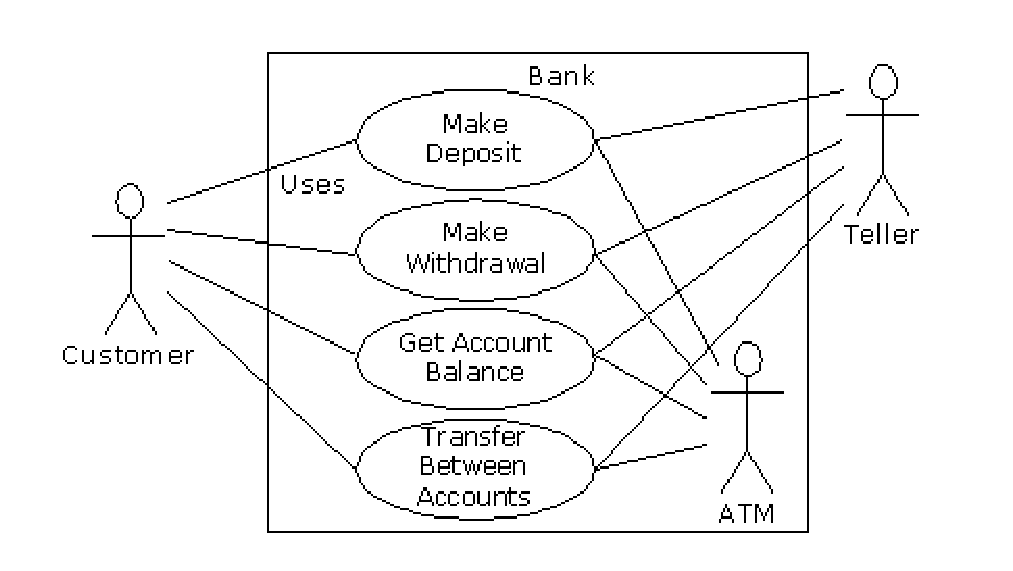
\includegraphics[scale=0.8]{eps/TIJ212.eps}
\end{figure}

上圖的每一個棒狀小人,都代表某個「參與者(actor)」,可以是真人,
也可以是某種形式的代理人(agent)。甚至可能是其他電腦系統,例如本例的
ATM(自動提款機)一樣。方格代表系統的邊界,橢圓代表 use case,
那是系統所能執行的有用工作的描述語句。介於參與者和use cases
之間的直線,代表兩者的互動。

只要系統對使用者而言,長相的確如此,那麼無論系統實際的實作方式為何,
都不會帶來影響。

即使底層系統十分複雜,use case 也沒有必要極度複雜。
其目的只是要顯示使用者所看到的系統的一面。例如:

\marginpar{\fbox{78}}
\begin{figure}[htbp]
\centering
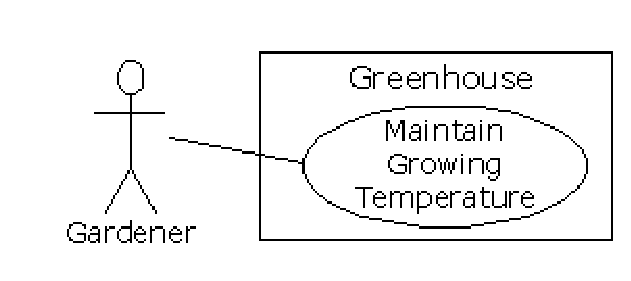
\includegraphics[scale=0.8]{eps/TIJ213.eps}
\end{figure}

use cases 會藉著「找出使用者在系統中可能存在的所有互動情形」而產生需求規格。
試著找出系統中完整的一組use cases,一旦完成,系統功能核心便在你的掌握之中。
專注於use cases 的好處是,它能讓你回歸本質面,
讓你免於陷入那些「無法對工作的達成產生關鍵影響」的因素。也就是說,
如果你擁有了一組完整的use cases,你便有能力描述你的系統,
並有能力進展到下一個階段。或許第一次嘗試時你無法徹底理解,但是不打緊,
所有事物都會即時顯現自己。再說,如果你想要在這個時間點上得到一份完美的系統規格,
最後不免陷入膠著。

如果你真的陷入膠著,可以使用粗略的近似工具,來發動這個階段的工作:
以些許數小段文字來描述系統,同時找尋其中的名詞和動詞。名詞可用以提示參與者、
use case 的環境(context,如上例之大廳)、或是在此 use case 中被操作的人工製品。
動詞可用以提示參與者和use case 之間的互動關係,並指出
use case 中的諸多步驟。你當然也會發現,在設計階段中,
名詞和動詞還可以對應至物件及訊息(但請注意,use case
描述的是子系統之間的互動關係,因此「名詞和動詞」這種技巧僅能做為腦力激盪工具,
無法用來產生use case)\footnote{關於use case,在 Schneider 與 Winters
合著的《Applying Use Cases》(Addison- Wesley 1998)以
及Rosenberg 所著的《Use Case Driven Object Modeling with UML》
 (Addison-Wesley 1999)兩本書中,有更詳盡的解說。} 。

介於use case 和參與者之間的邊界,可以指出使用者介面(UI)的存在,
但不定義任何使用者介面。關於使用者介面的定義及建造過程,請參考
Larry Constantine 和 Lucy Lockwood 合著,1999 年由 Addison-Wesley Longman
出版的《Software for Use》一書,或是親 訪www.ForUse.co網站。

雖然這是一種魔術,\marginpar{\fbox{79}}但是在這個時間點上制定一些基本時程規畫,
還是挺重要的。現在,你已對所要發展的東西有一些概括認識,因此,
對於所需花費的時間,你或許能夠捕捉到一些想法。許多影響因素開始在此處發酵。
如果你估計的時程過長,公司可能決定不開發(如此便能更合理地將資源用於它處 -
這是一件「好事」)。也許某位經理已經評估過此專案所需的時程,並試著影響你的評估。
喔,最好一開始就對時程保持誠實的態度,並儘早處理這個燙手山芋。
許多人嘗試建立精確的時程評估技巧,但或許最好的方法就是仰賴你自己的經驗和直覺。
先憑直覺來估計所需時間,再將它乘以兩倍,最後再加百分之十。你的直覺或許正確,
讓你可以及時完成專案。乘上兩倍是為了把事情做得更像樣,
最後的百分之十則用在潤飾處理上\footnote{對此,我的觀點後來又有所改變。
乘以兩倍再加上百分之十,雖然可以得到合理的估計 (假設不存在太多 wild-card 因子),
但是你仍舊得辛勤工作,才能在時限內完成工作。如果你需要時間以求更精緻的結果,
並在過程中得到樂趣,那麼我相信正確的倍數應該是 3 或4。}。 不論你怎麼解釋,
不論你在呈現如此時程時有著什麼樣的抱怨和運用,最後的結果似乎就是這樣。

\subsection{階段2:如何建立? (Phase 2: How will we build it?)}
在這個階段中,你必須完成設計,其中必須描述classes 的長相、以及 classes
之間的互動方式。「類別 - 責任 - 協同合作關係( Class- Responsibility -
Collaboration,CRC)」卡片在classes 及其互動關係識別上,是個極佳技巧。
這個工具的價值,部份來自於它的技術單純性:只需一組空白的3x5 卡片,寫上一些東西,
便可開張大吉。每張卡片都代表一個class,卡片必須寫上:

\begin{enumerate}
\item class 的名稱。這個名稱很重要,它得反映出class 的行為精髓,令
人望而生義。
\item class \marginpar{\fbox{80}} 的責任(responsibilities),也就是它應做的事情。
通常可以從其成員函式的簡要陳述中獲得
(這些函式名稱應該具備清晰的描述力),但也不排除其他註記。
如果你想要在這個過程中播種以求收穫,那麼,請從一個懶惰的程式員的角度來檢視問題:
「你會期盼怎樣的物件神奇般地出現,一舉解決你的問題?」
\item classes 的「協同合作(collaborations)」關係:哪些classes 會和這個
class 互動?互動(interact)是個意念廣泛的詞彙,它可能是指聚合關係
(aggregation),或只是很簡單地存在某些物件,提供服務給此一
class 的物件。協同合作關係應該考慮到class 的閱聽者。舉個例子,如果你建立起名為
Firecracker(鞭炮)的class, 那麼誰會觀察(observe)它呢?一個Chemist
(化學家)?或是一個Spectator(觀賞者)?前者想知道哪些化學材料可製造鞭炮,
後者能夠說出鞭炮爆炸時的顏色和形狀。
\end{enumerate}


\fbox{%
\begin{minipage}{.93\textwidth}
譯註:CRC card 是Kent Beck 和Ward Cunningham 於1989 年的
OOPSLA ( Object-Oriented Programming Systems, Languages and
Applications ) 學術研討會中, 以一篇《A Laboratory for Teaching
Object-Oriented Thinking》論文提出的。在Timothy Budd 所著的《An
Introduction to Object-Oriented Programming 2nd Edition》(Addison-
Wesley 1997)中有不錯的應用範例。
\end{minipage}%
}
\bigskip

你可能會覺得卡片應該大一點,好讓你可以從中取得你想要的所有資訊。
但它們的小尺寸其實是刻意的,不僅希望讓你的class 保持精巧,
也希望你不要太早鑽進太深的細節中。如果這般小卡片上的資訊無法滿足你的需求,
那就意謂這個class 太過複雜(如果不是因為你考慮得太仔細,就是應該產生更多的
classes 來因應)。理想的class 應該一眼就被了解。CRC card 的出發點,
就是要協助你準備第一份設計方案,以利全貌的取得,同時回過頭來修繕原先的設計。

溝通,是CRC card 帶來的眾多好處之一。最好是不要依賴電腦,在群體中即時完成溝通。
每個人都負責數個 classes (一開始可能沒有 classes 名稱,也沒有其他資訊),
一次解決一個「腳本」,決定哪些訊息會被發送給哪些不同的物件以符合腳本內容,
這樣就彷彿置身於一部生命模擬器中。當你經歷此一過程,你會逐一察覺需要動用哪些
classes、其責任為何、以及它們之間的合作關係。最終你便能填滿卡片中的欄位。
一旦你遍行所有 use cases,一份相當完備的初始設計方案就出爐了。

有一次我和某個開發團隊合作,他們從來沒有以\marginpar{\fbox{81}}
OOP 方式開發過專案。我站在他們面前,在白板上畫出各種物件。
為他們提供設計方案初稿的此次經驗,是我在使用 CRC card 之前,
最為成功的一次諮詢經驗。我們討論著物件應當用什麼方式彼此溝通,然後擦掉某些物件,
以其他物件替代。其實我只不過是把所有 CRC cards 都放在白板上罷了。該團隊
(也就是知道整個專案應該做些什麼事的人) 實際產生了設計內容;
他們真正「擁有」了這份設計。我只不過是藉著詢問適當問題、嘗試建立假設、
接收團隊回饋訊息以修正假設等種種方法,導引整個過程的進行。
整個過程最美好的地方莫過於,該團隊並非透過「對某些抽象範例的探討」
來學習物件導向設計,而是專注於他們最感趣味的設計之上。

當你準備好一組 CRC cards 時,你可能會想要使用UML\footnote{對新手而言,
我推薦先前提過的《UML Distilled, 2nd edition》。}
來為你的設計內容建立更正規的描述。這並非必要,但還是有幫助,
特別是當你想要將圖示投射到牆上,好好沉思一番時。UML 之外的另一個替代方案是
「物件和其介面的文字性描述語句」,甚至可以是「程式碼本身」\footnote{Python
(www.python.org)通常被用來做為「可執行的虛擬碼(pseudocode)」。}
(視程式語言而定)。

UML 也針對系統的動態模型,提供額外的圖示符號。當系統或子系統的狀態移轉行為,
重要到必須以專屬圖示加以表現時(例如在控制系統中), 這些符號就十分有用。
一旦資料成了具支配性的影響因素(例如資料庫),
你可能也需要描述系統和子系統內的資料結構。

當你完成了物件和其介面的描述,你就會知道階段2 的工作已告一段落。
嗯,其實這只是大部份的物件而已,仍然有一些遺漏掉了,得等到階段 3 才有辦法知道。
但這不礙事兒,你只要注意最終是否能夠發掘出所有物件就好了。
雖說若能在整個過程中愈早發掘出來最好,但 OOP 提供了足夠的結構,
因此即使晚一點才發掘出來也不會造成什麼負面影響。事實上在程式發展的過程中,
物件的設計應該發生於五個階段。

\subsubsection{物件(Object)設計的五大階段}
\marginpar{\fbox{82}}
物件的設計並不侷限於程式撰寫時期。事實上物件的設計動作會發生在一連串階段之中。
抱持這樣的看法,對你將大有幫助,因為你不會期盼馬上得到完美的結果,你會意識到,
對物件的行為、外貌長相的理解,是隨著時間而發生的。
這樣的觀點能夠應用於不同類型的程式設計上;某個特定型態的樣式
(pattern)會在一次又一次與問題對抗的過程中浮現出來
(這是《Thinking in Patterns with Java 》一書的主題, 該書可
www.BruceEckel.com 下載)。物件當然也有它們自己的樣式,在了解、
使用、重複運用物件的過程中,便會一一顯現出來。

\begin{enumerate}
\item 物件的發掘。這個階段發生在程式內部分析期間。透過對以下事項的檢視,
包括外在因子和邊界、系統中的元素重複情況、最小概念單元,便可能發掘出物件。
如果你已有一組class libraries,那麼某些物件的存在就很明顯。我們可以透過
classes 之間的共通性來訂定base classes,繼承關係也許此刻就會明朗,
也許還要等到設計後期。
\item 物件的組合:實地發展物件時,你會發現你得增加許多發掘期間未曾出現的新成員。
這些物件的內部需求,可能需要其他 classes 的援助。
\item 系統的建構。這個階段中將出現對物件的更多需求。就像學習過程一樣,
你的物件會逐步演化。由於得和系統中的其他物件溝通和接駁,因此可能得改變對
classes 的需求,甚至加入新的classes。舉例來說,你可能會發現需要動用某些諸如
linked list 之類的輔助性classes,它們包含很少狀態
(state),甚至不含任何狀態,只是用來輔助其他 classes 的運作。
\item 系統的延伸。當你將新功能加入系統,你可能會發現,先前的設計無法輕易擴充。
因此,你或許可以重新建構系統的部份組成,或許是加入新的 classes,或甚至新的
classes hierarchies。
\item 物件的重複運用。\marginpar{\fbox{83}}
對 class 而言,這無疑是最真實的考驗。
如果某人試著將物件重複運用於某個全新情境之中,他也許會找出某些缺點。
每當你更動一個class 以適應更多新程式,那個 class 的一般性原則就會變得更清楚。
最後你終於擁有真正可重複運用的 type - 可以讓大部份物件於特定系統發揮效用。
「可重複運用的types」彼此之間不甚具有共通性,而且,為了被反覆運用,
它們得解決較一般性的問題。 
\end{enumerate}

\subsubsection{物件(Object)發展的指導原則}
上述幾個階段,在你發展 classes 的思路上提供了一些指導原則:

\begin{enumerate}
\item 為特定問題產生一個class,然後讓它在解決其他問題的同時,
漸漸成長茁壯而趨於成熟。
\item 記住,發掘你所需要的classes 和其介面,是系統設計的主要工作。
如果所需的classes 俱已存在,那麼這個專案再簡單不過了。
\item 別強迫自己一開始就要知道所有事情;耐心地一面前進一面學習。
無論如何這都是比較愉快的方式。
\item 開始寫程式;讓某部份先動起來,好讓你可以驗證你的設計,
或是找出設計的盲點。別怕被那些和義大利麵條沒兩樣的程序式
(procedural style)程式碼逼上死路。classes 能夠切割問題,
對於控制無序與混亂很有助益。糟糕的classes 不會拖累優秀的classes。
\item 永保單純。物件若能夠保持小而簡潔,並提供明顯易懂的功能,
絕對比大而無當、介面繁複的對手來得好。每當面臨抉擇,請使用
Occams 的所謂剃刀法 (Razor approach):在眾多選擇中挑出最單純的一個,
因為最單純的classes 永遠是最好的。從小而簡潔出發,
當你更加了解class 的介面特性,便可加以擴充。隨著時間推移,我們很難將元素自
classes 中移除。
\end{enumerate}

\subsection{階段3:打造核心 (Phase 3: Build the core)}
這個階段進行初次轉換,將原始設計轉換為「對於可測試之程式碼的主體部份」
的編譯與執行動作。這麼做能夠驗證架構的正確性,
或找出錯誤所\marginpar{\fbox{84}}在。這當然不會只是一個回合而已,
這是一個開端,後續一系列步驟將能夠來回反覆地建造出系統,一如你在階段 4 中所見。

我們的目標是找出系統架構的核心,這個核心必須完成 - 不論一開始它是多麼地不完整 -
以便產出可運行的系統。你所產生的正是日後賴以為根基的框架
(framework)。你還會進行首次的系統整合與測試,並給予投資者一些訊息,
讓他們知道系統的長相大概是什麼樣子,系統目前的進展又是如何。
理想情況下你還會接觸到某些關鍵性風險。你或許也會察覺出原始架構中可更動、
可改善的地方,這些都是「不做就學不到」的東西。

系統建立過程中,包含對系統進行真實的檢查,也就是依據需求分析和系統規格
(不論以何種形式存在)進行測試。請確認你的測試動作對於需求和
use cases 皆進行了檢驗。系統的核心一旦穩固,也就等於做好了準備,
可以繼續往前進,並加入更多功能。
\subsection{階段4:use cases 的迭代 (Phase 4: Iterate the use cases)}
一旦核心架構能夠運作,你所加入的每一個功能組,本身都可視為一個小型專案。
你會在所謂「迭代(iteration)」過程中將功能組加入。這個迭代過程,
只佔整個發展期相當小的一段時間。

\bigskip
\noindent
\fbox{%
\begin{minipage}{\textwidth}
譯註:迭代 (iteration)是指一種反覆往返的概念。這裡的迭代過程中,
我們發展一個新功能,把它整合到先前系統,加以測試。接著再發展另一個新功能、整合、測試...。如此不斷地反覆往返,系統益形增長。
\end{minipage}
}
\bigskip

一次迭代過程有多大?理想情形下每個迭代過程持續進行一至三週
(隨著程式語言而有不同)。這個過程的最後,你會有一個整合妥當、經過測試的系統,
其功能較先前版本更豐富了。特別有趣的是迭代過程的歸依所在:單一
use case。每個 use case 都是一整套相關功能,
這些功能是你想要在單一迭代過程中加入系統的。這不僅讓你對 use case
的涵蓋範圍有了更好的認識,也讓你得以印證
use cases 的觀念。即使在分析和設計之後,
這個觀念也不應該被丟棄,因為在軟體發展過程中,無論哪一個階段,
它都是最根本的單元。

當你完成你所設定的全部功能\marginpar{\fbox{85}},或是外部期限已到,
而顧客也對現有版本感到滿意,便是上述迭代過程停止的時刻。
(請記住軟體是一種「預訂」
行業。)由於整個過程是反覆往返的,所以你有很多出貨機會,而非只能在單一點上;
如果你的專案採行開放源碼(open-source)策略,在這種反覆往返、
高度倚賴回饋訊息的環境中,能夠如魚得水地獲得成功。

迭代式發展過程,因為許多因素而顯得彌足珍貴。
帶有重大影響的風險可以被提早察覺並加以解決,顧客有足夠機會改變他們的想法,
程式設計者可以獲得更高的成就感,也可以更精準地掌控專案的進行。
除此之外還有個好處,那就是對投資者的訊息回饋,
讓他們可以看到產品中的每一樣事物的當前狀態。這麼做或許可以減少
(甚至完全去除)那些叫人傷透腦筋的狀態回報會議,並能夠堅定投資者的信心,
增加來自投資者的協助。

\subsection{階段5:演化 (Phase 5: Evolution)}
這個階段相當於傳統發展週期中的「維護(maintain)」階段。
其中涵蓋所有零零總總的事情,包括「讓它可以像一開始就被期望的那樣」到
「加一些客戶忘了提到的功能」,甚至更傳統的「修正浮上檯面的臭蟲」和
「隨著需求增加,加入一些新功能」,都算在裡頭。
許多錯誤的認知都被附加於「維護」一詞,使它承擔了品質上的某些欺瞞行為。
部份原因是這個詞彙讓人認為,你的確建立了一個原始程式,
而你需要做的便是為它更換零件、上點機油、並避免生鏽。
或許我們應該選一個更好的詞彙來描述實際上發生的事情。

我選擇以「演化(evolution)」來替代「維護」\footnote{Martin Fowler
的《Refactoring: improving the design of existing code》
(Addison - Wesley 1999)一書(完全以Java 為範例),
至少涵蓋了一個以上的「演化」面向。}。
其意思是,由於無法在第一回合就讓每一件事正確無誤,所以我們需要一些迴旋空間,
一面學習一面回頭修正。隨著你的學習,也隨著對問題本質更加透澈的了解,
需要更正的地方或許不少。如果你能不斷演化,
直到完全正確,那麼你所展\marginpar{\fbox{86}}示的優雅便能取得成功 -
不論是短期或長期。演化,是讓你的程式從
「好」到達「了不起」的關鍵,也是那些「第一回合無法真正了解」
之問題變得清楚的關鍵。它同時也是你的 classes 從「僅適用於單一專案」演化為
「足堪重複運用」的關鍵。

「事事正確無誤」所指的,並非單只是讓程式根據客戶需求和use cases 來運作。
它同時也意謂,程式碼的內部結構對你來說饒富意義,感覺上服服貼貼地組合在一起,
沒有難搞的語法、過大的物件、也沒有任何醜陋的代碼。此外,
一旦程式結構面臨更動(那是生命週期中無法逃避的),要如何生存下去,
你得有自己的看法。如何使這些更動可以做得輕鬆、做得乾淨俐落,更要有自己的判斷。
這不是一朝一夕的功夫。你不僅得了解自己所建的系統,
更得了解程式如何演化(即我所稱的「改變的向度
(vector of change)」)。幸運的是,物件導向程式語言特別擅長支援此類
「持續性修改動作」,是的,由物件所形成的邊界,會主動保持結構免於毀壞。
物件導向 (OO) 程式語言讓你可以進行更動,而你的程式碼不致於處處崩裂
(對程序性程式來說「更動」可能是很嚴重的事)。事實上,提供「演化機制」是
OOP 最為重要的優勢。

有了演化機制,你可以先建立某些看起來近似心中構思的東西,
然後把它拿來和設定需求相比較,看看哪些地方不合要求。然後回過頭去修正、
重新設計、重新實作程式裡頭尚未正確的部份\footnote{這有點像是所謂的
「快速建立原型(rapid prototyping)」。在這種方式下,
你可以用快速但相對不那麼乾淨的方式建立一個原型系統,藉此獲得對此系統的了解。
然後再將原型系統丟棄,好好地重新打造。「快速建立原型」的問題在於,
人們往往捨不得丟棄原型系統, 而想以它為基礎繼續開發。但是你得注意,
由於其中結合了程序式編程方法 (procedural programming)
中「結構不足」的缺點,往往導致混亂,帶來高昂的維護成本。} 。
想出正確解法之前,
你或許得花上好幾次功夫才能解決整個問題,或問題的某一部份。(研究所謂設計樣式
(Design Patterns),對此將有助益。你可以在
《Thinking in Patterns with Java 》書中找到更多參考資料, 此書可自網站
www.BruceEckel.com 下載。)


演化\marginpar{\fbox{87}}也會發生於你正在建立系統的時候。
當你檢查系統是否符合需求,卻發現它並非你想要的東西時,就需要演化了。
當你的系統正在運作,然後你才發現其實你要解決的是另一個截然不同的問題,
這也需要演化。如果你認為這種形式的演化正在發生,那麼你應該歸功於自己,
因為你儘快完成了第一版本,才有辦法判斷它是否的確是你想要的東西。

最該銘記於心的重要事情是,預設情形下,如果你修改了某個class,其 super-classes
和 sub-classes 都應該仍然正常運作。你沒有必要恐懼修改
(尤其是當你已經有了一組測試單元,用來檢驗你所做的修改是否正確時,更無需害怕)。
修改不必然會帶來毀壞,不過,任何修改的結果都應該被限制在 subclasses 和 (或)
你所修改之class 的特定合作者內。
\section{取得成功}
當然,你不會在尚未將規畫仔細繪製下來之前,冒然地動手蓋起房子。
如果你蓋的只是露天平臺,或者只是狗屋,你的規畫也許不會煞費苦心,
但你仍然可能想要稍微描繪個草圖,為自己領路。軟體的發展已經走到了極端。
長久以來,人們並沒有好好地在他們的發展過程中進行結構性規畫,
於是大型專案接二連三地失敗。為了解決這種問題,我們終結了那些瞄準大型專案、
有著令人望而生畏的繁多結構與細節事務的方法論。這些方法論令人畏於使用 -
看起來就像會耗掉你的全部時間於文件撰寫上,使你抽不出時間來寫點程式
(這的確常常發生)。我希望我所指出的是一條中庸之道 - 一把可移動量度的尺。
儘情使用符合你自身需求(以及個性)的方法吧。不論你選擇的方式有多麼簡單,
比起毫無計畫而言,「某種」形式的計畫終究還是可以為你的專案帶來極大的改善。
記住,根據統計,超過百分之五十 (有些評估甚至認為是百分之七十)
的專案以失敗收場。

透過對計畫的遵循 (寧可選擇既簡單又簡短者),並在開始撰碼之前先好好設計結構,
你便會發現,所有的事情,相較於「馬上潛心鑽研、開始亂搞一番」,
是那麼輕易地可以兜在一起,毫不費力。你會得到無上的滿足。我的經驗是,
找出優雅的解決方案,能夠得到極深的愉悅,這種深度愉悅的層次與過去的經驗完全不同;
更像是一種藝術,而不單只是技術。
優雅的方法不只是無聊的消遣,它們總是能夠成功。
它們不但讓你的程式\marginpar{\fbox{88}}更易於建立、易於除錯,
也更易於理解和維護。而這正是經濟價值之所在啊。

\section{Extreme programming(XP)}
從唸研究所開始,我便斷斷續續研讀過不少分析和設計技巧。Extreme
Programming(XP)是我見過最激進、最讓人愉快的一種觀念。在 Kent Beck 所著的
《Extreme Programming Explained》(Addison-Wesley, 2000) 書以及
www.xprogramming.com 網站上,都有對此觀念的闡述。

XP 是程式設計工作上的一種哲學,也是一組實踐準則。
其中某些準則已反映於晚近問世的其他方法論中。XP 最重要、最獨特的貢獻,就我看來,
便是「測試優先(write tests first)」和「搭檔設計(pair programming)」 兩者。
雖然 Beck 強烈主張完整過程,但他也指出,即使只採用上述兩條實作準則,
還是可以大幅提高開發工作的生產力和穩定度。
\subsection{測試優先 (Write tests first)}
傳統上,測試往往被歸為整個專案的最末枝節,在「每件事情都正常運作」之後才被考慮,
其價值只是為了「確認真的沒有問題」。
這種想法使得大家潛意識裡把測試視為一件低優先權的工作。
專門從事測試的人沒有獲得足夠的地位,而且常常被隔離在地下室,
遠離那些所謂「真正的程式研發人員」。測試團隊則回敬說:
『我們就像穿著黑袍,把東西弄壞了就樂不可支。』老實說,
當我找出編譯器的瑕疵時也有相同的感覺。

XP 讓測試工作和程式撰寫平起平坐(甚至有更高的優先權),
這種想法是一種革命性的轉變。事實上你得在撰寫待測程式碼之前,先寫好測試樣例,
而後這些測試樣例便永遠與程式碼同在。每次進行專案整合動作時
(那很頻繁,甚至可能一天兩次),所有測試樣例都必須能夠成功執行。

「測試優先」可以產生兩個極為重要的影響。

首先,這麼做能夠強迫人們把\marginpar{\fbox{89}}
class 的介面定義清楚。當人們試著進行系統設計時,我常常建議他們
「幻想有個能夠解決特定問題的完美 class」做為可用工具。
XP 的測試策略又更向前跨了一步,它明確指出 class
對其使用者而言應該具備怎樣的外貌,同時也明確指出
class 必須有的行為模式。直截了當,毫不含糊。你可以寫下一堆文件、
或是產生所有想要的圖示,來描述 class 應有的行為模式及其外觀長相,
但沒有什麼東西比一組測試來得更為真實。前者像一紙清單,後者卻是一紙契約,
一紙由編譯器與程式共同遵守的契約。
很難有其他東西能夠比一組測試樣例更具體地描述一個 class 了。

產生測試樣例時,你被迫對 class 進行完整而詳細的考量,
並常常因此發現一些需要加入的功能,這些功能也許可能在「以UML 圖、CRC 卡、
use cases 等方式做為思考進行路線」的過程中漏失。

「測試優先」的第二個重大影響是,你得在每次做出一份軟體成品時,
都將所有的測試樣例執行一遍。這麼做可以涵蓋整個測試環節的另一半,
也就是編譯器所主宰的部份。如果你從這個角度來看程式語言的發展,你會看到,
技術面上最實際的改善其實是以測試為中心:組合語言只檢查語法正確與否,
C 卻加進了某些對語義的限制,避免型別(types)被誤用。
OOP 語言加進的語義限制更多 - 如果你把這些限制視為某種形式的測試的話。
「資料型別是否被妥善運用」和「函式是否被正確呼叫」
都是由編譯器和執行期系統所進行的測試。
我們已經看到了這些測試內建於程式語言後的結果:人們能夠撰寫更複雜的系統,
並讓它們運作無誤,但所花費的時間和力氣卻更少了。我曾對此苦思許久,
現在我意識到,上述動作都是測試:你有可能弄錯一些東西,
而內建測試功能的安全網會告訴你,有問題發生,並指出問題所在。

但是「自程式語言本身的設計切入,藉以提供內建測試機能」,所能做的也就這麼多了。
某些情形下你得適時介入,補足完整測試的缺口,藉以對你的程式進行整體檢驗。
難道你不希望像編譯器不時從旁照料一般地,
讓\marginpar{\fbox{90}}這些測試樣例一開始就能夠適時派上用場嗎?
這也就是你之所以必須「先寫下測試樣例,並在每次做出一份軟體成品後便自動執行測試」
的原因。 如此一來,你的測試樣例便能成為程式語言所提供之安全網的延伸。

使用那些愈來愈具威力的程式語言時,我發現一件事情:
由於我知道這些語言有能力使我不必耗費時間於程式臭蟲的捕捉,
所以我愈來愈敢嘗試一些尖銳的實驗。 XP 的測試體系對整個專案來說,所做之事亦同。
因為你知道你的測試樣例,絕對有能力捕捉到你所引入的所有問題,
所以你可以在任何必要的時候,進行大幅度修改,不必憂心整個專案陷入混亂狀態。
這真是太有威力了。
\subsection{搭檔設計 (Pair programming)}
我們向來被諄諄教誨,嚴守個人主義。在學校裡頭,成敗都操之在己。與左右鄰居合作,
就被視為「作弊取巧」。媒體,尤其好萊塢電影,也告訴我們,
英雄總是反抗無知的服從\footnote{雖然有點大美國主義,
但是好萊塢的故事的確流傳各地。} 。搭檔設計 (pair programming)
悖離這種強烈的個人主義。程式員常常被視為個體存在的典範- 就像 Larry Constantine 
喜歡說的「牛仔撰碼員(cowboy coders)」。XP 背棄這種想法,
認為應該兩個人合用一部工作站合夥寫程式才對。而且寫程式的環境應該是
「在一大塊空間裡頭擺一堆工作站」,不應該在其中樹立室內設計師最喜歡的隔板。
事實上,Beck 說,如果想皈依 XP,第一件事情應該是拿起螺絲起子、L 形鈑手,
把所有造成阻礙的東西通通拆\footnote{包括 (特別是) 擴音裝置。
我曾經在某家公司任職,這家公司強烈要求,打給所有業務主管的每一通電話,
都必須加以廣播。這麼做時常打斷我們的工作。管理者無法想像,
擴音裝置這麼「重要」的服務,有多麼讓人受不了。趁著四下無人,
我最後剪掉了擴音機的電線。} 。(那麼當然就得有個經理級的人物,
有能力移轉來自設備部門的忿怒囉)

搭檔設計(pair programming)\marginpar{\fbox{91}}
的價值在於,當某個人思考,另一個人就實際撰碼。
從事思考的那個人得將整體宏觀牢記於心 - 不僅僅是對手邊的問題徹底了解,
同時還得熟記 XP 的諸般實踐準則。舉例來說,兩個人一起工作,
就不太可能會有一個人跳出來說:「我可不想先寫測試樣例。」
如果一人陷入困境,兩個人就可以交換角色。如果兩人都陷入困境,
那麼他們兩人發呆的樣子,可能會被整個工作區中的某個可以幫得上忙的人發現。
這樣子搭檔工作,可以讓事情更平順,並依計畫前進。不過,或許更重要的是,
這樣子能讓程式設計變得更與人互動,更充滿樂趣。

我已經在我的某些研討會的習題中加入搭檔設計理念,而我發現,
這似乎相當程度地改善了每一個人的經驗。
\section{Java 為什麼成功}
Java 能夠取得如此的成功,原因在於其目標的設定:
為當今開發人員解決他們所面臨的諸多問題。提高生產力是 Java 的終極目的。
生產力來自於許多層面,但是 Java 語言希望從語言層面提供儘可能的協助。
Java 的目的在實用;Java 語言的根本考量,就是為程式員爭取最多的利益。
\subsection[易於表達、易於理解的系統]{易於表達、易於理解的系統\\
Systems are easier to express and understand}
被設計用來「與待解問題相稱」的class,先天上就有較佳的表述能力。
這意謂當你撰寫程式碼時,並不使用電腦術語 - 亦即解域 (solution space)
空間中的術語,而是以題域空間(problem space)中的術語來描述解法。
如此一來便能夠以高階觀念來處理問題,而且每一行程式碼可以做的事情就更多了。

易於表達所帶來另一好處便是維護,
而維護佔了整個程式生命週期中極大的成本比例
(如果那些數據報告可信的話)。如果程式易於理解,便相對地易於維護。
這也同時可以降低文件撰寫與維護的成本。

\subsection{透過程式庫(libraries)發揮最大槓桿效應}\marginpar{\fbox{92}}

開發程式的最快途徑,就是使用現成的東西:程式庫(library)。Java 的主要目標之一,
便是讓程式庫的使用更容易。「將程式庫轉換為新的 data types (classes)便是
Java 達成此一目標的手段。因此,引入程式庫,意謂將新的 types 加到程式語言裡頭。
由於Java 編譯器會留意程式庫被使用的方式 -
保證初始化動作和清除動作確實正確地執行,並確保呼叫函式的方式合乎規矩 -
你可以專注於程式庫的運用,而不必擔心如何製造它們。

\subsection{錯誤處理}
「錯誤處理」在 C 裡頭向來是個聲名狼藉的問題,而且常被忽略 -
只能祈求上天給你好運。如果你所開發的程式很大,很複雜,
那麼大概沒有什麼事比得上「程式某處暗藏一個錯誤,
我們卻對其發生原因毫無頭緒」還要糟糕吧。 Java 的異常處理
(exception handling) 便是「一旦發生錯誤,保證一定通知你,
並讓你採取一些處理動作」的機制。
\subsection{大型程式設計}
對於程式的大小和複雜度,許多傳統語言都存在若干內建限制。以 BASIC 為例,
它對一般等級的問題,有著最棒的快速解決方案。但是當程式的長度超過數頁,
或是逾越該語言的標準題域之外,你就會像「在一池黏稠液體中游泳」一樣,動彈不得。
你所使用的程式語言何時會失去作用?噢, 沒有一條明白的界線。即使存在界線,
你還是會忽略它。因為你總不能說:「我的 BASIC 程式現在太大了,我得重新用
C 寫過!」所以你會試著硬塞幾行進去,藉以增加新功能。
就這樣不知不覺付出了額外的成本。

Java 具備大型程式設計能力- 也就是抹除了小程式和大程式之間的複雜度界線。
如果你只是想寫一個 "Hello World" 小程式,當然不需動用 OOP,
但是當你需要用到時,這些功能唾手可得。而且編譯器會積極找出臭蟲所在,
不論對小程式或大程式,一律如此。

\marginpar{\fbox{93}}
\section{過渡策略 (Strategies for transition)}
如果你大量採用 OOP,那麼你的下一個問題可能是:「我要如何才能夠讓我的上司、
同事、部門、同儕們都開始使用物件呢?」想想你,一個獨立的程式員,
如何開始學習一個全新的程式語言和一個全新的設計思維?其實你辦到了。
首先是訓練和範例教學,然後是試驗性的專案,讓你感受一些基本原理,
而不需要做一些頭昏眼花的事情。接下來就是一個「真實世界」中的專案,
這個專案真的能夠做一些有用的事情。在此專案過程中,
你不斷閱讀、向高手請教、和朋友交換心得,藉以持續進行學習。
這就是有經驗的程式員轉換到 Java 跑道時可以採取的方式。當然,想要轉換整個公司,
必然會造成一定程度的群體變動,但是請記住,個人所採取的方式,
仍舊可以在每一個步驟中派上用場。
\subsection{實踐準則}
想要過渡到 OOP 和 Java,可以參考以下建議的實踐準則:
\begin{enumerate}
\item 訓練
\

第一步便是某種形式的教育。別忘了公司在程式碼上的投資,
並且努力不要讓任何事情處於混亂狀態超過六到九個月 -
雖然每個人都對介面運作的方式感到困惑。挑選一小群人來進行教育,
這一小群人最好是個性好奇、 能夠彼此合作、能夠在學習
Java 的時候彼此奧援的人。

有時候我也會建議另一種作法,一次教育公司裡的所有階層,
包括對決策高層的概觀性說明,以及對專案開發者的設計和撰碼課程。
這種方式特別適合小型公司進行根本性的移轉,或是對大型公司的部門層次來進行。
不過,由於這會帶來較高的成本,所以也有人選擇從專案層次的訓練開始,
先做個前導性專案(可能邀請外聘講師),再讓專案中的成員變成公司其他成員的老師。

\item 低風險專案\marginpar{\fbox{94}}
\

先以低風險專案做為試探,並允許錯誤發生。獲得些許經驗之後,
便可以將這個前導團隊的成員播種到其他專案去,或把他們視為 OOP 技術支援幕僚。
第一個專案可能無法一蹴而成,所以不應該挑選會對公司產生重大影響的案子。
這個專案應該簡單、能自我控制、具啟發性 - 意謂這個專案應該產生某些
classes,對公司其他人開始學習Java 時帶來一些意義。
\item 向成功借鏡
\

起跑之前,先找一些有著良好物件導向設計的範例出來閱讀。通常,有相當的機會,
別人早已解決了你的問題。就算沒有人恰巧解決你的問題,你也有可能應用所學,
修改他人設計的抽象方法,套用在自己的需求上。這也就是設計樣式
(design patterns)的一般概念。《Thinking in Patterns with Java》
一書涵蓋這個主題,你可以自 www.BruceEckel.com 下載。
\item 使用既有的程式庫 (libraries)
\

更換跑道至 OOP,經濟上的主要動機便是能夠以 class libraries 的形式,
輕鬆地重複運用既有的程式碼(本書廣泛使用的 Java 標準程式庫更是如此)。
當你能夠把既有的程式庫當做基礎,建立物件並加運用,便能產生最短的程式開發週期。
不過某些程式設計新手可能無法意識到這一點,也可能沒有發現到程式庫的存在,
抑或過度迷戀程式語言的魅力,總想自己動手寫一些早已存在的 classes。
如果你能夠早點在這個過渡過程中努力找出他人所寫的程式碼,並加以重複運用,
就能夠透過 OOP 和 Java,取得最大的成功。
\item 不要以 Java 重寫既有的程式
\

將那些既有的、函式風格的程式碼,重新以 Java 寫過,
對時間而言通常不是最佳運用方式。如果你一定得把它們轉向物件形式,你可以運用
Java 原生介面 (Java Native Interface),用以和 C 或 C++ 程式接軌。
本書附錄 B 對此介面有所討論。這麼做可以得到漸進的好處,
特別是當那些程式碼被選定重複運用時。不過這麼一來,
可能你就無法在剛開始的幾個專案中\marginpar{\fbox{95}}看到驚人的生產力提升 -
這一點唯有在全新專案中才有可能出現。Java 和 OOP 的出眾,
最能夠表現在讓一個專案的概念成真、落實。
\end{enumerate}

\subsection{管理上的障礙}
如果你是一個管理者,你的工作便是為你的團隊爭取資源、
排除所有影響團隊成功的障礙,並試著提供最能帶來生產力、
最讓人樂在其中的工作環境,讓你的團隊成為最有可能展現奇蹟的團隊,
達成那些不可能的任務。 遷移至 Java 平台所需付出的成本,
會落在以下所列的三個範疇內。如果這並不會讓你付出什麼代價,那真是太好了。有些
OOP 替代方案,是專門為 C 程式員 (或其他程序式語言的使用者)
所組成的團隊量身提供的。雖然,相較於那些替代方案,遷移至 Java
平台所需付出的代價,顯然低廉多了,但不論再怎麼低廉的成本,依舊不能不花任何成本。
此外,在嘗試將 Java 推廣到你的公司之前、在著手進行遷移計畫之前,
你得先知道路上可能有的一些絆腳石,才好應付。
\subsubsection{起動成本}
遷移至 Java 平台,所需的成本,不單只是取得Java 編譯器而已
(Sun Java 編譯器是免費的,所以這談不上是顆絆腳石)。如果你願意投資在訓練上面
(可能得請專家為你的第一個專案提供顧問諮詢),
並且找到了可解決你的問題的程式庫並加以購買,
而不是試著自己重新開發這些程式庫,那麼你的中長期成本會降至最低。
這些都是得花費實際金錢的成本, 必須納入專案提案書。此外,可能有一些隱藏成本,
來自於「新語言的學習」和「可能導入的新設計環境」所引起的生產力損耗。
訓練和顧問諮詢無疑能夠將這些成本降到最低,
但是團隊成員也必須克服他們自身在了解新技術時湧現的掙扎。在這個過程中,
他們會犯下更多錯誤 (這也是一種特色,因為大家都公認錯誤是通往學習的捷徑) ,
而且生產力降低。儘管如此,面對某些類型的問題,即便大家還只在學習
Java 的過程中,還是有可能比「停留於 C 的使用」帶來更好的生產力 (雖然,
所犯的錯誤或許更多,每天所完成的程式碼或許更少)。
\subsubsection{效能問題}\marginpar{\fbox{96}}
一個常被問到的問題是:「OOP 不會將我的程式變得既肥且慢嗎?」這個問題的答案是:
「視情況而定。」 Java 所提供的額外安全功能,傳統上是犧牲諸如 C++
語言所具備的效能而來的。諸如 ``hotspot'' 之類的技術和編譯器的技術,
多數都能夠大幅提高執行速度;此外還有更多致力於效能提升的努力,正在持續進行。

如果你關注的事情集中在「快速建立原型」上面,你可以匆匆將所有組成拼湊起來,
略去效能上的考量。如果你使用的是其他廠商提供的程式庫,
它們通常都已經由供應商最佳化了,因此在快速開發模式下,效能通常不是問題所在。
當你已經擁有一個想要的系統,如果它夠小而且夠快,你的工作就算告一段落。
如果不是這樣,你就得開始使用一些效能研判工具
(profiling tool)來進行調整,看看能否改寫小部份程式以提高速度。如果不行,
就得找找看有沒有什麼修正手法可以施行於底層,使上層程式碼不需要隨之更動。
一旦這些方法都束手無策,你才需要更改設計。由於效能在設計中佔了極重要的地位,
所以效能必須成為設計良窳的評量依據之一。藉由快速開發方式,
提前找出效能的癥結所在,可以帶來好處。

如果你發現某個函式正是效能瓶頸所在,你可以 C/C++ 重寫那個函式,
並以 Java 原生函式 (native methods)與之接軌,這個主題見本書附錄 B。
\subsubsection{常見的設計錯誤}
一旦你的開發團隊採用 OOP 和 Java,程式員通常會經歷一連串常見的設計錯誤。
通常是因為早期專案的設計和實作上沒有從專家那兒取得足夠的回饋訊息。
這可能是因為沒有在公司內培養出專家,也可能是因為存在著對固定顧問諮詢的反對聲浪。
很容易就可以感受到你是否在整個週期中過早了解 OOP,並走偏了方向。有些事情,
對熟悉此語言的人來說平淡無奇,對新手而言卻是十分重大的討論議題。
藉由經驗豐富的外聘專家提供訓練與顧問諮詢,可以避免許多傷害。

\section{Java vs. C++?}\marginpar{\fbox{97}}
Java 看起來很像C++,而且如此成熟,似乎應該有足夠的份量取而代之。
不過我開始質問這種思考邏輯。畢竟 C++ 仍然具備了某些 Java 沒有的特色,
而且雖然有許多承諾顯示 Java 終有一天會和 C++ 一樣快,甚至更快,
甚至我們也看到了一些效能上的持續進展,但是並沒有什麼驚人突破。再者,
整個程式開發環境仍然對 C++ 有持續性的關注,所以我不認為 C++
會在任何可見的近期內消失。 (程式語言似乎永遠隱而不退。在我的某次
Java 中/高階研討會上,Allen Holub 宣稱,目前最被廣泛使用的兩個語言分別是
Rexx 和 COBOL。)

我於是開始思考 Java 的長處,其戰場其實和 C++ 稍有不同。C++
這個語言並不試著為某種類型的問題量身打造。一般而言它可融入許多不同的方法,
解決種種問題。有些 C++ 工具將程式庫、組件模型
(component models)、程式碼產生工具 (code-generation tools) 結合在一起,
藉以解決視窗環境下 (例如 Microsoft Windows) 及終端用戶相關的應用程式發展問題。
但是,Windows 開發市場中最被廣泛使用的工具是什麼? 是
Microsoft Visual Basic(VB) - 儘管 VB 所產生的程式碼類型,
會在程式長度超過數頁之後就變得難以管理
(而且其語法肯定讓人感到困惑)。即便
VB 如此成功、如此受歡迎,在程式語言的設計上,它不是一個好範例。
如果能夠同時擁有 VB 的單純和威力,又不會產生一堆難以管理的程式碼,
那就真是太好了。這也正是為什麼我認為 Java 會大紅大紫的原因:
它是「下一個 VB」。你可能會、也可能不會害怕聽到這樣的說法,但是請想想,那麼多的
Java 功能,都是為了讓程式員更容易解決一些諸如網絡、
跨平台使用者介面之類的應用層次上的問題,更別說它還具備了語言本身的設計,
允許極大型而具彈性的程式碼開發工作。再加上一點: Java
具備了我所見過的程式語言中最穩固的型別檢查和錯誤處理機制,
你可以飛快提升程式設計的生產力。

那麼,你應該在專案中以 Java 替代 C++ 囉?除非是 Web 上的 applet,
否則你應該考慮兩個因素。首先,如果你想使用現成的大量 C++ 程式庫
(而\marginpar{\fbox{98}}且你將從那兒獲取相當多的生產力),
或者如果你已經有了現成的 C 或 C++ 程式碼,那麼 Java 可能會減緩你的開發時程,
不會帶來速度的提升。

如果你基本上是從頭開始發展所有的程式碼,那麼 Java 特性之中遠勝於
C++ 的「單純性」,便會大幅縮短你的開發時程。有許多傳言(我從一些原本使用
C++ 後來轉投Java 陣營的開發團隊聽來的),認為可以帶來兩倍的速度提升。如果
Java 的效能弱點對你而言不重要,或如果你可以其他方法加以補償,那麼在純粹的
「市場到位時間」考量下,很難不選擇 Java。

最大的問題還是在效能。使用最原始的 Java 解譯器, Java 大概比 C 慢上 20 到50 倍。
這一點隨著時間已有大幅改進,但仍然有著相當巨大的差距。談到電腦,無非就是速度。
如果電腦帶給你的服務沒有快上太多,或許你寧願手動完成。
(我曾經聽過有人建議,如果你需要較快的執行速度,你可以先用 Java
獲得較短的開發時間,再以某種工具及其所支援的程式庫,將那些 Java 程式碼轉換為
C++。)

使 Java 足堪適用於大多數專案,關鍵來自於執行速度的提升,例如所謂
「just-in time(JIT)」編譯器、Sun 推出的「hotspot」技術、乃至於原生碼
(native code)編譯器。當然,原生碼編譯器無法吸引那些需要跨平台執行能力的人,
但它帶來的執行速度卻足以逼近 C 和 C++。而且以 Java 寫成的程式,
要進行跨平台編譯,比起 C 和 C++來說真是簡單太多了。
(理論上你只需要重新編譯。不過以前也有一些程式語言做過相同的承諾。)

你可以在本書第一版附錄中找到 Java 和 C++之間的許多比較,以及對 Java 的現實觀察。
(本書所附光碟片中有第一版電子書,你也可以從 www.BruceEckel.com 下載)
\section{摘要}
本章試著讓你體驗一下 OOP (物件導向程式設計) 和 Java 中廣泛的議題,包括:
OOP 為何如此與眾不同、 Java 又為何如此格外出眾、 OOP
方\marginpar{\fbox{99}}法論的概念。最後更涵蓋了「當你的公司遷移到
OOP 和 Java 平台時,會遇到的種種問題」。

OOP 和 Java 不見得適用於每個人。重要的是評估你自己的需求,並決定
Java 是否能夠在滿足這些需求上得到最佳結果,抑或使用另一套程式設計系統
(包括你正在使用的那一套)對你來說比較好。
如果你知道你的需求在可預見的未來會非常特殊,而 Java 可能無法滿足某些特定限制,
那麼你應該再考察其他方法\footnote{我特別推薦你看看
Python(http://www.Python.org)}。
即使你最後選擇了 Java,你至少還得了解有那些項目可供選擇,
並對於為什麼選擇這個方向有非常清楚的看法。

你知道,程序式程式 (procedural program) 看起來是什麼樣子:
就是資料的定義和函式的呼叫。想知道此類程式的意義,你得花上一些功夫,
從頭到尾檢視那些函式呼叫和低階概念,才能夠在心中建立起一套模型。
這也就是為什麼我們在設計程序式程式時,需要一些中介表達方法,
因為這種程式天生就容易混淆人們的認知,是的,它們用以表達的詞彙,太偏電腦,
不像是你解決問題時所用的術語。

在你能夠找到的程序式語言的所有功能之上, Java 又添加了許多新觀念。
因此,你自然而然會假設, Java 程式中的 main() 遠比 C 裡頭的兄弟複雜許多。
關於此點,你會感到十分驚喜。妥善撰寫的 Java 程式,通常遠比同等性質的 C
程式更單純,更容易理解。你只需查看那些「用來表示題域空間中的概念」
(而非任何電腦表述方式) 的所謂物件,以及那些在物件之間傳遞的訊息
(用來代表題域空間中的活動) ,就可以輕鬆掌握整個 Java 程式。
OOP 的最大樂趣在於,面對妥善設計的程式,只需加以閱讀,
很容易就可理解程式碼的內容。事實上,通常不會有太多程式碼,
因為許多問題都已經透過「重複運用既有程式庫」的方式解決掉了。
